%%%% autodd_icdm26.tex

\typeout{ICDM--26 AutoDD Paper}

% TeX Live 2025's tabular/array rework clashes with IEEEtran.cls's \@@array patch;
% roll the LaTeX kernel back to a compatible release (2023-11-11 is chosen so that
% xcolor is not also rolled back). Remove if the class is updated.
\RequirePackage[2023-11-11]{latexrelease}
\documentclass[conference]{IEEEtran}
\IEEEoverridecommandlockouts

\usepackage{cite}
\usepackage{amsmath,amssymb,amsfonts}
\usepackage{amsthm}
\usepackage[linesnumbered,ruled,vlined]{algorithm2e}
\usepackage{graphicx}
\usepackage{textcomp}
\usepackage{xcolor}
\usepackage{url}
\usepackage[hidelinks]{hyperref}
\usepackage{orcidlink}
\usepackage[utf8]{inputenc}
\usepackage{booktabs}
\usepackage{float}
\usepackage{multirow}
\usepackage{array}
\usepackage[caption=false,font=footnotesize]{subfig} % \subfloat; caption=false keeps IEEEtran's own caption style

\urlstyle{same}

\def\BibTeX{{\rm B\kern-.05em{\sc i\kern-.025em b}\kern-.08em
    T\kern-.1667em\lower.7ex\hbox{E}\kern-.125emX}}

% Per CPS editor (M. Nunez, 2026-08-29): omit page numbers and any copyright
% information at the bottom of pages -- CPS adds these during processing.

\title{AutoDD: Learning to Select Drift Detectors for Evolving Data Streams}

% For double-blind review, comment out the author block below and use the
% anonymous one. The real author block is provided for the camera-ready.
%\author{\IEEEauthorblockN{Anonymous}}

\author{
\IEEEauthorblockN{Nilesh Verma\,\orcidlink{0009-0006-4705-6169}\textsuperscript{1}, Albert Bifet\,\orcidlink{0000-0002-8339-7773}\textsuperscript{1,2}, Bernhard Pfahringer\,\orcidlink{0000-0002-3732-5787}\textsuperscript{1}, Maroua Bahri\,\orcidlink{0000-0002-7420-7464}\textsuperscript{3}}
\IEEEauthorblockA{\textsuperscript{1}\textit{AI Institute, University of Waikato}, Hamilton, New Zealand \\
\textsuperscript{2}\textit{T\'el\'ecom Paris, Institut Polytechnique de Paris}, Paris, France \\
\textsuperscript{3}\textit{CNRS, LIP6, Sorbonne Universit\'e}, Paris, France \\
\{nilesh.verma, albert.bifet, bernhard.pfahringer\}@waikato.ac.nz, maroua.bahri@lip6.fr}
}

\begin{document}

\maketitle

\begin{abstract}

Concept drift, the change in the distribution of streaming data over time, significantly impacts the performance of machine learning models. While numerous drift detection methods have been proposed, selecting and configuring the most suitable detector for a specific data stream remains a challenging task. Existing AutoML frameworks for streaming data that automate model selection rely on fixed drift detection strategies, leaving a critical gap in automation. This paper introduces \textit{AutoDD} (\underline{Auto}mated \underline{D}rift \underline{D}etector), a novel framework that jointly automates detector selection and hyperparameter configuration using a hierarchical learning approach. AutoDD extracts comprehensive online meta-features and employs a two-level hierarchical selection algorithm to adaptively choose both the detector and its configuration. Experiments on ten synthetic and real-world datasets show that AutoDD consistently outperforms state-of-the-art detectors while maintaining computational efficiency.

\end{abstract}

\begin{IEEEkeywords}
concept drift detection, algorithm selection, contextual bandits, online meta-learning, data streams
\end{IEEEkeywords}

\section{Introduction}

Concept drift, where the statistical properties of streaming data evolve over time, poses a significant challenge in data stream mining \cite{Gama2014Survey,Bifet2010MOA}, incremental learning \cite{Losing2018IncrementalOnline}, and non-stationary learning \cite{Lu2019Learning}. As data distributions change, machine learning models experience degraded performance, necessitating timely detection and adaptation. This phenomenon manifests in various forms, including sudden (abrupt) drift, gradual drift, incremental drift, and recurring drift. For instance, an electricity price prediction model may encounter sudden drift when market regulations change abruptly, experience gradual drift as consumer behaviour shifts over seasons, or observe recurring drift driven by daily demand cycles~\cite{Lu2019Learning}.

% \begin{figure}[!ht]
%     \centering
%     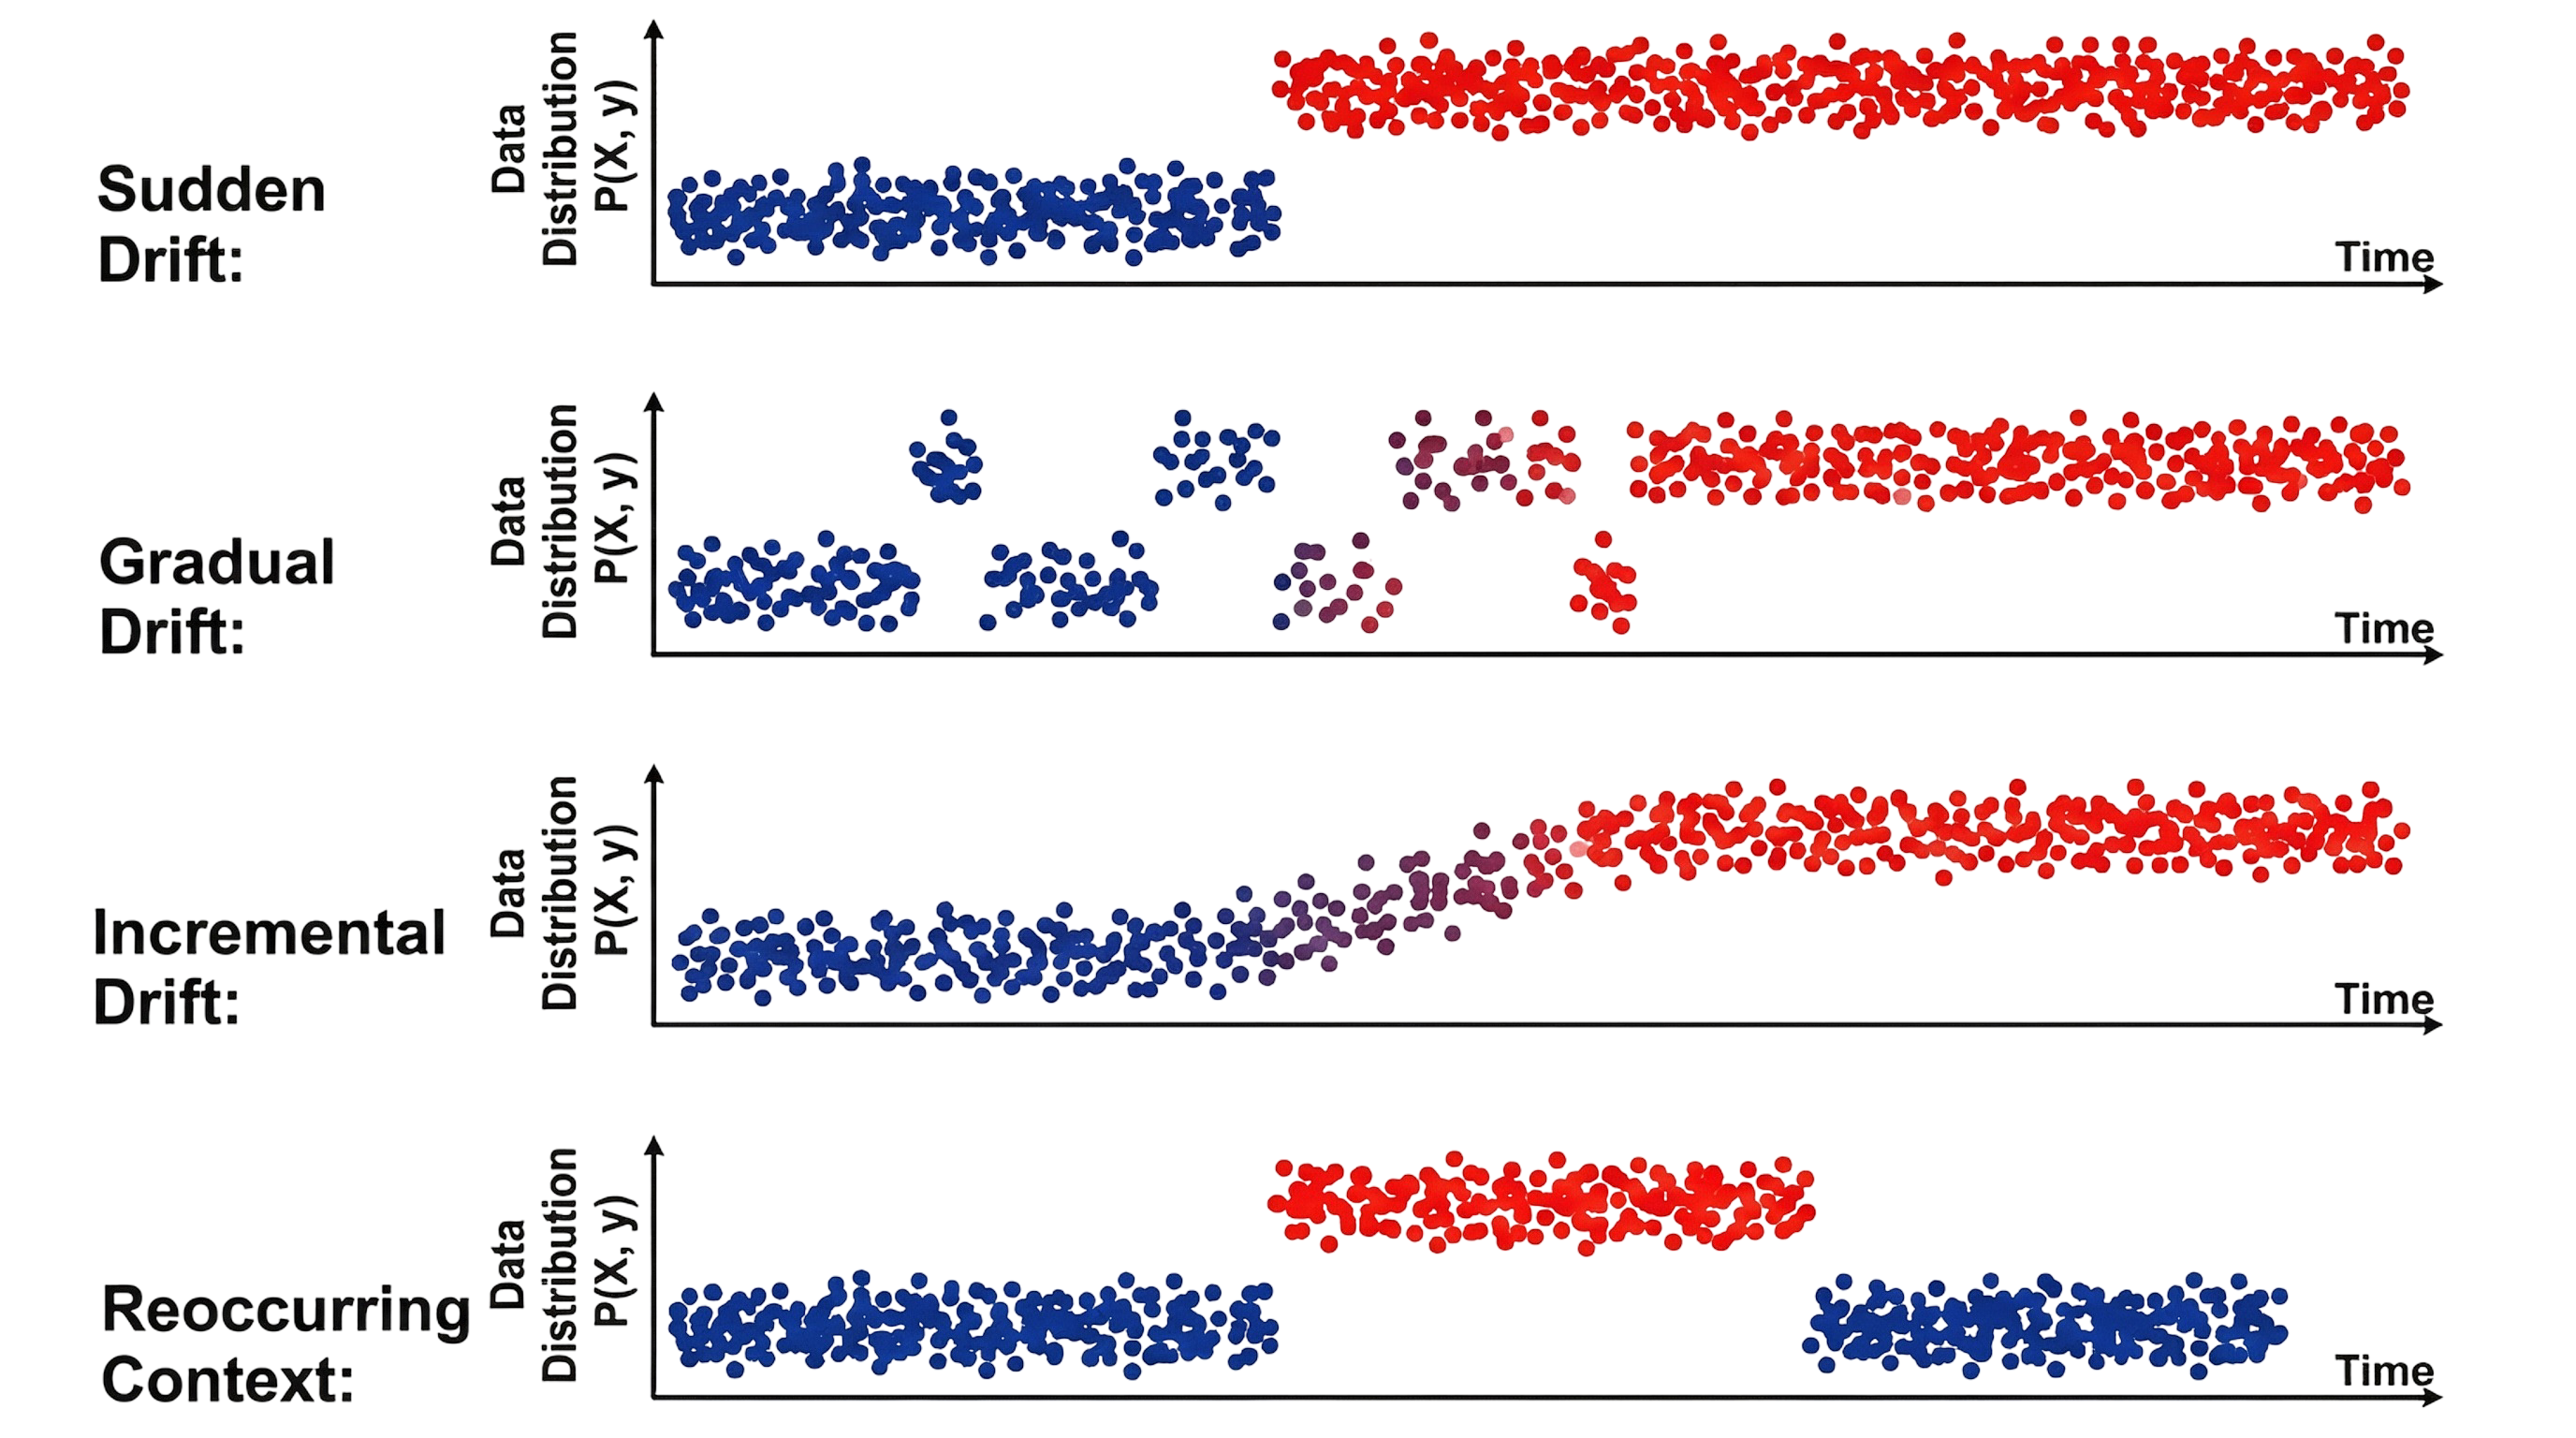
\includegraphics[width=0.85\columnwidth]{images/concept/type_of_drift_detection.png}
%     \caption{Types of concept drifts, following the taxonomy of Lu et al.~\cite{Lu2019Learning}.}
%     \label{fig:type_of_drift}
% \end{figure}

Over the past two decades, numerous drift detection methods have been developed to address this challenge \cite{Gama2014Survey,Lu2019Learning}, spanning error rate-based \cite{Gama2004DDM,Bifet2007ADWIN,Pesaranghader2017MDDM}, distribution-based \cite{Kifer2004ChangeDetection,Raab2020KSWIN}, uncertainty-based \cite{Lu2025PUDD}, and meta-learning \cite{Yu2021MetaADD} paradigms. Yet no single detector performs best across all conditions \cite{Gama2014Survey,Souza2020Benchmark}, because each embeds assumptions about how drift manifests. As a result, a detector well suited to abrupt changes may respond slowly to gradual ones \cite{BaenaGarcia2006EDDM,Lu2019Learning}, and the most appropriate choice can shift as the stream itself evolves \cite{Souza2020Benchmark}. However, a fundamental challenge remains unresolved in systematically selecting and configuring the most appropriate drift detector for a given data stream.

Automated Machine Learning (AutoML) has revolutionised the field by addressing similar selection challenges in batch learning scenarios \cite{Hutter2019AutoML}. Recent advancements have extended AutoML to streaming data, enabling automatic selection and configuration for supervised learning tasks \cite{Celik2023OAML,Verma2024ASML}. However, these systems treat drift detection as a fixed component, requiring manual specification and leaving a critical gap in the automation framework.

Automating this choice online is challenging because drift labels are unavailable as the stream arrives \cite{Gama2014Survey,Lu2019Learning}, so detector quality must be inferred from a proxy reward derived from downstream model behaviour rather than from ground-truth change points \cite{Bifet2007ADWIN,Yu2021MetaADD}, and because the joint space of detectors and their configurations is too large to search as a single flat action set \cite{Hutter2019AutoML}. Unlike detector ensembles that run and combine many detectors at once \cite{Barros2018,Alippi2017Hierarchical}, or meta-learning methods that learn a fixed mapping offline \cite{Yu2021MetaADD}, an effective solution must select and configure one detector online and continually refine this choice as the stream evolves. To bridge this gap, we introduce \textit{AutoDD} (\underline{Auto}mated \underline{D}rift \underline{D}etector), a modular framework that automates drift detector selection and configuration using a hierarchical learning approach, compatible with any model or AutoML pipeline. Figure~\ref{fig:framework} gives an overview of the framework. AutoDD makes three main contributions.

\begin{itemize}
\item We propose \textit{AutoDD}, a novel framework for automated drift detector selection and configuration in evolving data streams.
\item AutoDD formalises the problem of joint detector and hyperparameter selection and solves it via a two-level hierarchical bandit using online meta-features, LinUCB \cite{Li2010LinUCB} for detector selection, and Thompson Sampling \cite{Agrawal2012Thompson} for hyperparameter configuration.
\item A comprehensive experimental study across ten benchmarks shows that AutoDD ranks first on mean accuracy and macro-F1 against state-of-the-art detectors, while maintaining computational efficiency.
\end{itemize}

The remainder of this paper is organised as follows. Section~\ref{sec:related} reviews related work, Section~\ref{sec:problem} defines the problem, and Section~\ref{sec:method} presents AutoDD and its theoretical analysis. Sections~\ref{sec:experiments} and~\ref{sec:results} describe the experimental setup and results, while Sections~\ref{sec:discussion} and~\ref{sec:conclusion} discuss limitations and conclude the paper.

\begin{figure*}[t]
    \centering
    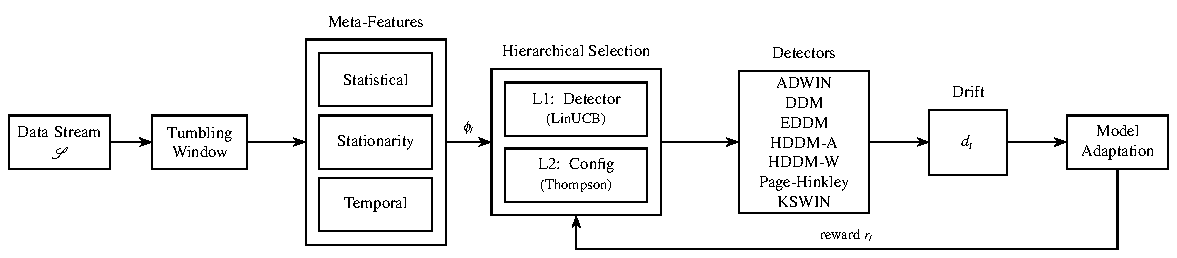
\includegraphics[width=0.95\textwidth]{images/framework/framework_tikz.pdf}
    \caption{Overview of AutoDD. A window buffer forms context $\boldsymbol{\phi}_t$ from statistical, stationarity, and temporal meta-features. LinUCB selects a detector and Thompson Sampling selects its configuration. The detector emits drift signal $d_t$, which triggers model adaptation, and reward $r_t$ updates both levels.}
    \label{fig:framework}
\end{figure*}


\section{Related Work}
\label{sec:related}

Drift detection methods can be broadly categorised into three paradigms. \textbf{Error rate-based methods} monitor fluctuations in classifier error rates, triggering alarms when changes are statistically significant. DDM \cite{Gama2004DDM} pioneered the warning-drift framework by monitoring prediction accuracy under binomial distribution assumptions, followed by EDDM \cite{BaenaGarcia2006EDDM} which focuses on distances between errors to detect gradual drift, HDDM \cite{FriasBlanco2015Hoeffding} which applies Hoeffding's inequality with exponentially weighted moving averages, and ADWIN \cite{Bifet2007ADWIN} which maintains adaptive sliding windows that automatically shrink when distribution changes are detected. Page-Hinkley \cite{Page1954Continuous} applies cumulative sum control charts to detect mean shifts in sequential data. Recent advances include MDDM \cite{Pesaranghader2017MDDM}, which uses McDiarmid's inequality for shorter detection delays with tighter concentration bounds, and ADDM \cite{Mayaki2022ADDM}, which models error rates as SETAR time series \cite{Tsay1989TestingAM} to achieve lower false alarm rates. \textbf{Distribution-based methods} compare data distributions across windows by quantifying dissimilarity between new and historical data distributions \cite{Kifer2004ChangeDetection}, including approaches based on information theory \cite{Dasu2006InformationTheoretic}, competence models \cite{Lu2014CompetenceModels}, and the Kolmogorov-Smirnov test (KSWIN) \cite{Raab2020KSWIN} which detects changes in univariate feature distributions. KSWIN is a recent representative of the statistical two-sample test family, which also includes earlier detectors such as IKS \cite{dosReis2016IKS} and WRS \cite{Barros2018}. \textbf{Uncertainty and learning-based methods} address limitations of error-rate monitoring. PUDD \cite{Lu2025PUDD} leverages prediction confidence for earlier detection by monitoring changes in prediction uncertainty distributions, while Meta-ADD \cite{Yu2021MetaADD} employs prototypical networks to classify drift types via meta-learning on diverse drift scenarios.

Recent developments in automated algorithm selection and hyperparameter optimisation (CASH) \cite{Hutter2019AutoML} have been extended to streaming scenarios~\cite{kulbach2022evolution}. However, these streaming AutoML systems automate supervised task selection while assuming a fixed, manually specified drift detector, so the detector itself is never selected or configured automatically. AutoDD addresses this gap by bringing the detector into the automation loop, learning online which detector and configuration best suit the current stream.

\section{Problem Formulation}
\label{sec:problem}

We consider a supervised data stream in which instances arrive sequentially and potentially without end. At each time step $t$, the stream produces an instance $(\mathbf{x}_t, y_t)$, where $\mathbf{x}_t \in \mathbb{R}^{d_{\mathrm{in}}}$ is the feature vector and $y_t$ is its label, drawn from a joint distribution $P_t(\mathbf{x}, y)$. The stream $\mathcal{S}$ exhibits concept drift when this distribution changes over time, that is, when
\begin{equation}
\mathcal{S} = \{(\mathbf{x}_t, y_t)\}_{t=1}^{\infty}, \qquad \exists t, t' : P_t(\mathbf{x}, y) \neq P_{t'}(\mathbf{x}, y).
\end{equation}

Given a detector portfolio $\mathcal{D} = \{D_1, \ldots, D_K\}$ where each $D_i$ has configuration space $\mathcal{H}_i$, AutoDD addresses the streaming detector selection and configuration problem. Inspired by the CASH formulation \cite{Hutter2019AutoML}, we jointly optimise the detector choice and its hyperparameters:
\begin{equation}
\label{eq:cash}
\resizebox{0.95\columnwidth}{!}{$
(D^*_t, \boldsymbol{\eta}^*_t) = \arg\max_{D_i \in \mathcal{D}, \boldsymbol{\eta} \in \mathcal{H}_i} \mathbb{E}[\mathrm{Perf}(D_i(\boldsymbol{\eta}), \mathcal{S}_t) \mid \boldsymbol{\phi}_t]
$}
\end{equation}
where $\boldsymbol{\phi}_t\in\mathbb{R}^m$ is the context, $\mathcal{S}_t$ is the stream segment, and $\mathrm{Perf}(\cdot)$ is downstream model performance. Hereafter $[K]=\{1,\ldots,K\}$, and $t$ indexes window-level selection rounds rather than individual arrivals.

\section{Automated Drift Detector}
\label{sec:method}

AutoDD employs an adaptive, closed-loop architecture to dynamically select and configure drift detectors. This architecture operates through several key steps. First, the system initialises the detector portfolio with standard hyperparameters and sets up the learning parameters. During online operation, meta-features characterising stream velocity, stationarity, and temporal patterns are continuously extracted from the incoming data stream. These meta-features serve as context for the LinUCB agent, which selects a detector from the portfolio. Thompson Sampling then chooses a hyperparameter configuration for the selected detector. The configured detector monitors the stream and triggers model adaptation upon detecting drift. Finally, performance feedback is computed based on detection outcomes, which updates both the LinUCB and Thompson Sampling components to refine future selections. Algorithm~\ref{alg:autodd} formalises this adaptive learning cycle, which enables AutoDD to improve its detector selections over time.

\begin{algorithm}[t]
\caption{AutoDD}
\label{alg:autodd}
\KwIn{Stream $\mathcal{S}$, portfolio $\mathcal{D}$, window size $w$; exploration $\alpha_{\text{ucb}}$, regularisation $\lambda_{\text{reg}}$, configurations $C$, prior $(a_0,b_0)$, reward constants $(\rho_{\mathrm{tp}},\kappa,\rho_{\mathrm{fp}},\rho_{\mathrm{fn}},\rho_{\mathrm{tn}},\tau_{\text{drop}})$}
\KwOut{Window-level drift signals $\{d_t\}_{t=1}^{\infty}$}
Initialise $\mathbf{A}_i \gets \lambda_{\text{reg}}\mathbf{I}_m$, $\mathbf{b}_i \gets \mathbf{0}$ for all $i \in [K]$\;
Initialise $a_{i,c} \gets a_0$, $b_{i,c} \gets b_0$ for all $i \in [K], c \in [C]$\;
Initialise model $\mathcal{M}_0$, window buffer $W \gets \emptyset$\;
\ForEach{instance $(\mathbf{x}_n, y_n) \in \mathcal{S}$}{
    $W \gets \operatorname{tail}_w(W \cup \{(\mathbf{x}_n, y_n)\})$\;
    \If{$|W| = w$ and $n \bmod w=0$}{
        $\boldsymbol{\phi}_t \gets \textsc{Extract}(W)$ \tcp*{meta-features}
        \For{$i = 1$ \KwTo $K$}{
            $\text{UCB}_i \gets \boldsymbol{\phi}_t^\top \hat{\boldsymbol{\theta}}_i + \alpha_{\text{ucb}} \sqrt{\boldsymbol{\phi}_t^\top \mathbf{A}_i^{-1} \boldsymbol{\phi}_t}$ \tcp*{$\hat{\boldsymbol{\theta}}_i = \mathbf{A}_i^{-1}\mathbf{b}_i$}
        }
        $i_t \gets \arg\max_i \text{UCB}_i$ \tcp*{select detector}
        \For{$c = 1$ \KwTo $C$}{
            Sample $\psi_{i_t,c} \sim \text{Beta}(a_{i_t,c}, b_{i_t,c})$\;
        }
        $c_t \gets \arg\max_c \psi_{i_t,c}$ \tcp*{select configuration}
        $d_t \gets D_{i_t}(\boldsymbol{\eta}_{i_t,c_t}).\textsc{Detect}(W)$\;
        \If{$d_t = 1$}{
            $\mathcal{M}_t \gets \mathcal{M}_0$ \tcp*{reset model}
        }
        Compute reward $r_t$ using Eq.~\eqref{eq:reward}\;
        $\mathbf{A}_{i_t} \gets \mathbf{A}_{i_t} + \boldsymbol{\phi}_t \boldsymbol{\phi}_t^\top$;\quad $\mathbf{b}_{i_t} \gets \mathbf{b}_{i_t} + r_t \boldsymbol{\phi}_t$\;
        $\tilde{r}_t \gets (r_t + 1)/2$\;
        $a_{i_t,c_t} \gets a_{i_t,c_t} + \tilde{r}_t$;\quad $b_{i_t,c_t} \gets b_{i_t,c_t} + (1-\tilde{r}_t)$\;
    }
}
\end{algorithm}

\subsection{Algorithm Overview}

AutoDD executes one selection cycle every $w$ arrivals using the current $w$-instance window, beginning with meta-feature extraction.

\textbf{Meta-Feature Extraction:} The $m=15$ features are statistical (velocity, dimensionality, sparsity, noise, and class imbalance), stationarity-based (error volatility, KL divergence, autocorrelation, mean shift, and variance shift), or temporal (trend, periodicity, change frequency, change magnitude, and recurrence). After finite-value replacement and clipping, $\ell_2$ normalisation yields $\boldsymbol{\phi}_t\in\mathbb{R}^m$ with $\|\boldsymbol{\phi}_t\|_2\leq1$; Appendix Table~\ref{tab:metafeatures} gives the estimators.

\textbf{Detector Portfolio:} AutoDD maintains $K$ window-, error-, and distribution-based detectors. Table~\ref{tab:portfolio} gives their hyperparameters and ranges. For detector $i$, candidate set $\{\boldsymbol{\eta}_{i,c}\}_{c\in[C]}\subset\mathcal{H}_i$ contains the literature default and $C-1$ configurations sampled on the stated scale, where $[C]=\{1,\ldots,C\}$.

\begin{table}[t]
\centering
\caption{Detector portfolio with hyperparameter configurations.}
\label{tab:portfolio}
\resizebox{\columnwidth}{!}{%
\small
\begin{tabular}{|l|l|l|l|l|l|}
\hline
\textbf{Detector} & \textbf{Type} & \textbf{Parameter} & \textbf{Range} & \textbf{Scale} & \textbf{Default} \\
\hline
ADWIN & Window-based & $\delta_{\text{adwin}}$ & [0.0001, 0.1] & log & 0.002 \\
\hline
\multirow{2}{*}{Page-Hinkley} & \multirow{2}{*}{Window-based} & $\theta_{\text{ph}}$ & [10, 100] & int & 50 \\
\cline{3-6}
& & $\delta_{\text{ph}}$ & [0.001, 0.01] & log & 0.005 \\
\hline
\multirow{2}{*}{DDM} & \multirow{2}{*}{Error-based} & $w_{\text{thresh}}$ & [1.5, 3.0] & linear & 2.0 \\
\cline{3-6}
& & $d_{\text{thresh}}$ & [2.0, 4.0] & linear & 3.0 \\
\hline
\multirow{2}{*}{EDDM} & \multirow{2}{*}{Error-based} & $\alpha_{\text{eddm}}$ & [0.90, 0.99] & linear & 0.95 \\
\cline{3-6}
& & $\beta_{\text{eddm}}$ & [0.85, 0.95] & linear & 0.90 \\
\hline
HDDM-A & Error-based & $\delta_{\text{hddm}}$ & [0.0001, 0.01] & log & 0.001 \\
\hline
HDDM-W & Error-based & $\lambda_{\text{hddm}}$ & [0.01, 0.1] & log & 0.05 \\
\hline
\multirow{2}{*}{KSWIN} & \multirow{2}{*}{Distribution-based} & $\alpha_{\text{ks}}$ & [0.001, 0.05] & log & 0.005 \\
\cline{3-6}
& & $w_{\text{ks}}$ & [50, 500] & int & 100 \\
\hline
\end{tabular}
}
\end{table}

\subsection{Hierarchical Learning Approach}

The two-level decomposition adapts detector choice and hyperparameter configuration jointly without treating all $K \times C$ detector-configuration pairs as a single flat action space.

\textbf{Level 1 - Detector Selection via LinUCB:} Context $\boldsymbol{\phi}_t$ describes the stream, the $K$ detectors are arms, and the proxy reward measures detection performance. LinUCB \cite{Li2010LinUCB} assumes
\begin{equation}
r_{i,t} = \boldsymbol{\phi}_t^\top \boldsymbol{\theta}_i^* + \epsilon_t
\end{equation}
where $\boldsymbol{\theta}_i^*\in\mathbb{R}^m$ is detector $i$'s unknown parameter vector. The algorithm selects the highest upper confidence bound:
\begin{equation}
\resizebox{0.9\columnwidth}{!}{$
i_t = \arg\max_{i \in [K]} \left( \boldsymbol{\phi}_t^\top \hat{\boldsymbol{\theta}}_{i,t} + \alpha_{\text{ucb}} \sqrt{\boldsymbol{\phi}_t^\top \mathbf{A}_{i,t}^{-1} \boldsymbol{\phi}_t} \right)
$}
\end{equation}
where $\hat{\boldsymbol{\theta}}_{i,t}=\mathbf{A}_{i,t}^{-1}\mathbf{b}_{i,t}$ is the pre-decision ridge estimate, with
\begin{equation}
\mathbf{A}_{i,t}=\lambda_{\text{reg}}\mathbf{I}_m+\sum_{s<t:i_s=i}\boldsymbol{\phi}_s\boldsymbol{\phi}_s^\top,\quad
\mathbf{b}_{i,t}=\sum_{s<t:i_s=i}r_s\boldsymbol{\phi}_s .
\end{equation}
Here, $\mathbf{A}_{i,t}\in\mathbb{R}^{m\times m}$ and $\mathbf{b}_{i,t}\in\mathbb{R}^m$ contain observations before round $t$; $\lambda_{\text{reg}}>0$ regularises the estimate and $\alpha_{\text{ucb}}>0$ controls exploration.

\textbf{Level 2 - Hyperparameter Selection via Thompson Sampling:} Given $D_{i_t}$, Thompson Sampling \cite{Agrawal2012Thompson} selects its configuration. Each $c\in[C]$ has Beta parameters $(a_{i,c},b_{i,c})$, initialised with prior $(a_0,b_0)=(1,1)$. We sample
\begin{equation}
\label{eq:ts_sample}
\psi_{i_t,c} \sim \text{Beta}(a_{i_t,c}, b_{i_t,c}) \quad \forall c \in [C]
\end{equation}
and select configuration:
\begin{equation}
\label{eq:ts_select}
c_t = \arg\max_c \psi_{i_t,c}
\end{equation}

After observing reward $r_t$, we update:
\begin{align}
\label{eq:ts_update}
a_{i_t,c_t} &\gets a_{i_t,c_t} + \tilde{r}_t \\
b_{i_t,c_t} &\gets b_{i_t,c_t} + (1 - \tilde{r}_t)
\end{align}
where $\tilde{r}_t = (r_t + 1)/2$ normalises the reward to $[0,1]$. %This cascading approach provides tractability (only $K$ arms at Level 1), specialization (each detector's hyperparameters tuned independently), and fast adaptation (Thompson Sampling quickly identifies effective configurations).

\subsection{Evaluation and Adaptation}

Without ground-truth drift labels, we use the downstream model's windowed prequential accuracy $a_t\in[0,1]$ to define the proxy reward
\begin{equation}
\label{eq:reward}
r_t = \begin{cases}
\rho_{\mathrm{tp}} + \min(\kappa\,\Delta a_t, \rho_{\mathrm{tp}}) & d_t=1, \Delta a_t > \tau_{\text{drop}} \\
-\rho_{\mathrm{fp}} & d_t=1, \Delta a_t \leq \tau_{\text{drop}} \\
-\rho_{\mathrm{fn}} - \min(\Delta a_t, \rho_{\mathrm{fn}}) & d_t=0, \Delta a_t > \tau_{\text{drop}} \\
\rho_{\mathrm{tn}} & d_t=0, \Delta a_t \leq \tau_{\text{drop}}
\end{cases}
\end{equation}
where $d_t\in\{0,1\}$ is the window-level alarm, $\Delta a_t=a_{t-1}-a_t$, and $\tau_{\text{drop}}$ is the accuracy-drop threshold. The $\rho$ terms name the four proxy outcomes and $\kappa$ scales the drop. With $\rho_{\mathrm{tp}},\rho_{\mathrm{fn}}\leq0.5$ and $\rho_{\mathrm{fp}},\rho_{\mathrm{tn}}\leq1$, the caps keep $r_t\in[-1,1]$. Window averaging and $\tau_{\text{drop}}$ reduce transient noise, although the reward remains coupled to the learner and labels; A4 states the fidelity needed to interpret proxy quality.

At selection boundary $n_t=tw$, an alarm resets the model, after which incremental learning resumes:
\begin{equation}
d_t=1:\ \mathcal{M}_{n_t}\gets\mathcal{M}_0,\qquad
\mathcal{M}_{n_t+s}\gets\text{Update}(\mathcal{M}_{n_t+s-1},(\mathbf{x}_{n_t+s},y_{n_t+s})),\ s>0.
\end{equation}

The implementation additionally updates Level~1 at alarms; Level~2 and the theory use window-boundary updates.

\subsection{Computational Complexity}
Using the estimators in Appendix Table~\ref{tab:metafeatures} and rank-one inverse updates, the per-window complexity excluding detector and learner costs is
\begin{equation}
T_{\mathrm{win}}=O(wd_{\mathrm{in}}+w\log w+Km^2+C),\quad
S_{\mathrm{win}}=O(Km^2+KC+wd_{\mathrm{in}}),
\end{equation}
where the FFT contributes $w\log w$, LinUCB contributes $Km^2$, and Thompson Sampling contributes $C$ time and $KC$ state.

\subsection{Theory}\label{sec:theory}

We analyse the two selection levels as idealised proxy-reward bandit sub-problems.

\textbf{Assumptions.} Let $\mathcal{G}_t$ contain the history and context available before round $t$'s reward. Following contextual-bandit analysis \cite{Abbasi2011Improved,Lattimore2020Bandit}, we assume:
\begin{itemize}
\item \textbf{(A1) Bounded features:} $\|\boldsymbol{\phi}_t\|_2\leq L$; our normalisation gives $L=1$.
\item \textbf{(A2) Linear reward:} For each detector $i$, some $\boldsymbol{\theta}_i^*\in\mathbb{R}^m$, $\|\boldsymbol{\theta}_i^*\|_2\leq S$, satisfies
\begin{equation}
\mathbb{E}[r_{i,t}\mid\mathcal{G}_t]=\boldsymbol{\phi}_t^\top\boldsymbol{\theta}_i^*.
\end{equation}
\item \textbf{(A3) Conditional noise:} $\epsilon_{i,t}=r_{i,t}-\boldsymbol{\phi}_t^\top\boldsymbol{\theta}_i^*$ is conditionally zero-mean and $\sigma_{\text{noise}}$-sub-Gaussian given $\mathcal{G}_t$; bounded rewards permit $\sigma_{\text{noise}}=1$.
\item \textbf{(A4) Proxy fidelity:} Expected proxy-reward and true-quality orderings agree across detector--configuration pairs under Eq.~\eqref{eq:cash}.
\end{itemize}

\emph{Remark (stationarity under drift).} A2 requires a stationary conditional reward map, not stationary $P_t$; context represents its changes. Rising proxy-oracle agreement in Appendix Table~\ref{tab:conv_main} is consistent with this approximation.

\textbf{Theorem 1 (Level 1 Proxy Regret).} Fix each detector's configuration and let $T$ count window-level rounds. Under A1--A3, confidence $\delta_{\text{conf}}\in(0,1)$ and radius
\begin{equation}
\resizebox{0.98\columnwidth}{!}{$
\alpha_T=\sigma_{\text{noise}}\sqrt{2\log\frac{K}{\delta_{\text{conf}}}+m\log\!\left(1+\frac{TL^2}{m\lambda_{\text{reg}}}\right)}+\sqrt{\lambda_{\text{reg}}}S,
$}
\end{equation}
the LinUCB rule with $\alpha_{\text{ucb}}=\alpha_T$ achieves, with probability at least $1-\delta_{\text{conf}}$,
\begin{equation}
\resizebox{0.95\columnwidth}{!}{$
R_1(T) = \sum_{t=1}^{T} \left( \max_{i} \boldsymbol{\phi}_t^\top \boldsymbol{\theta}_i^* - \boldsymbol{\phi}_t^\top \boldsymbol{\theta}_{i_t}^* \right) = \tilde{O}(m\sqrt{KT}).
$}
\end{equation}

\textit{Proof Sketch.} A union bound over arms and the self-normalised inequality \cite{Abbasi2011Improved} simultaneously give, for all arms and rounds,
\begin{equation}
\|\boldsymbol{\theta}_i^*-\hat{\boldsymbol{\theta}}_{i,t}\|_{\mathbf{A}_{i,t}}\leq\alpha_T.
\end{equation}
On this event the UCB rule bounds the instantaneous regret as
\begin{equation}
\max_i\boldsymbol{\phi}_t^\top\boldsymbol{\theta}_i^*-\boldsymbol{\phi}_t^\top\boldsymbol{\theta}_{i_t}^*\leq2\alpha_T\|\boldsymbol{\phi}_t\|_{\mathbf{A}_{i_t,t}^{-1}}.
\end{equation}
Applying the elliptical potential lemma \cite{Dani2008Stochastic} per detector and Cauchy--Schwarz across detectors gives
\begin{equation}
R_1(T)=\tilde{O}(m\sqrt{KT}). \tag*{$\square$}
\end{equation}

\textbf{Proposition 2 (Level 2 Proxy Regret).} Fix detector $i$ and let its configurations yield independent stationary rewards $\tilde r\in[0,1]$ with means $\mu_{i,c}$ and $\mu_i^*=\max_c\mu_{i,c}$. Under the Bernoulli-sampling reduction, Beta Thompson Sampling over a fixed $n$ plays satisfies
\begin{equation}
\mathbb{E}[R_{2,i}(n)]=\mathbb{E}\!\left[\sum_{s=1}^{n}(\mu_i^*-\mu_{i,c_s})\right]=O(\sqrt{Cn\log n}).
\end{equation}

\textit{Proof Sketch.} The standard $C$-armed result gives the displayed problem-independent bound \cite{Agrawal2013Further}. Our fractional Beta update (Eq.~\eqref{eq:ts_update}) replaces the sampled Bernoulli outcome by its expectation, so this is a surrogate for the idealised problem rather than a guarantee for the implementation. \hfill $\square$

The two results apply only to the idealised sub-problems and do not compose into joint detector--configuration regret. A4 preserves ordering only; it does not transfer a numerical proxy-regret rate to true quality. The experimental fixed $\alpha_{\text{ucb}}$ is tuned separately from $\alpha_T$.

\section{Experiments}
\label{sec:experiments}

\subsection{Datasets and Base Models}
We evaluate AutoDD on ten benchmark datasets comprising five synthetic and five real-world streams, with characteristics detailed in Table~\ref{tab:datasets}. To isolate drift detection performance from model selection effects, all methods use two fixed base models, GaussianNB and Hoeffding Adaptive Tree (HAT)~\cite{domingos2000mining}. These two learners represent fundamentally different model families (probabilistic and tree-based) and are the standard benchmark base learners used in the data stream mining literature~\cite{Bifet2010MOA,Barros2018}.

\subsection{Baselines}
We compare AutoDD against twelve baselines, namely a no-detector baseline and seven portfolio detectors (ADWIN, DDM, EDDM, HDDM-A, HDDM-W, Page-Hinkley, KSWIN). We also include four state-of-the-art methods, MDDM \cite{Pesaranghader2017MDDM}, ADDM \cite{Mayaki2022ADDM}, PUDD \cite{Lu2025PUDD}, and Meta-ADD \cite{Yu2021MetaADD}. All detectors use recommended hyperparameter settings from the literature. The portfolio includes one recent representative per detector family rather than every variant. Because AutoDD's selection mechanism is detector-agnostic, a larger portfolio extends only the action set, not the method.

\begin{table}[t]
\centering
\caption{Dataset characteristics (Multiple* = Sudden, Gradual, Incremental, and Recurring drift types)}
\label{tab:datasets}
\small
\begin{tabular}{|l|l|r|r|l|}
\hline
\textbf{Dataset} & \textbf{Type} & \textbf{Instances} & \textbf{Features} & \textbf{Drift Type} \\
\hline
SEA & Synthetic & 500,000 & 3 & Multiple* \\
HYP & Synthetic & 500,000 & 10 & Multiple* \\
AGR & Synthetic & 100,000 & 9 & Multiple* \\
RBF & Synthetic & 200,000 & 10 & Multiple* \\
RTG & Synthetic & 100,000 & 30 & Multiple* \\
Elec & Real-world & 45,312 & 8 & Unknown \\
Weather & Real-world & 18,159 & 8 & Unknown \\
Spam & Real-world & 4,601 & 57 & Unknown \\
Airlines & Real-world & 539,383 & 7 & Unknown \\
Poker & Real-world & 829,201 & 10 & Unknown \\
\hline
\end{tabular}
\end{table}

\subsection{Evaluation Protocol}
We measure prequential accuracy as the percentage of correct predictions using test-then-train evaluation~\cite{Bifet2010MOA}. On the synthetic streams we additionally report prequential macro-averaged F1 over the class labels under the same protocol. We stress that this is the F1 of the downstream classifier, not a drift-detection F1 scored against ground-truth change points. The benchmark includes continuously drifting streams such as HYP and RTG, for which no discrete ground-truth drift positions exist, so a detection-matching score is undefined here and we do not report one. For real-world datasets, we report the number of detected drifts (DN) instead. The two are complementary. Accuracy is dominated by the majority class, whereas macro-F1 weights classes equally and so exposes the minority-class collapse that follows when a detector adapts too late or resets too often. Neither scores detection timing directly, which we treat as a limitation of proxy-based evaluation. Following the benchmarking guidance~\cite{Souza2020Benchmark}, we interpret DN relative to the consensus detection range across methods rather than as an absolute target, treating values far above or below this range as over- and under-detection respectively.

\subsection{Implementation Details}
AutoDD uses all $m$ meta-features with a fixed window size, bandit parameters, and $C$ configurations per detector throughout. Results are averaged over 10 runs with random seeds uniformly sampled from the range [1, 100]. Implementation uses Python with River~\cite{Montiel2021River} on a MacBook Pro with Apple M2 Pro and 16GB RAM.\footnote{Code and datasets are available at \url{https://github.com/TechyNilesh/AutoDD}}

\section{Results}
\label{sec:results}

We conduct a comprehensive evaluation of AutoDD against classical detectors and state-of-the-art methods.

\begin{table*}[p]
\centering
\caption{Synthetic datasets under GaussianNB. Rank in ($\cdot$). \textbf{Bold} = best, \underline{underline} = second-best per column.}
\label{tab:synthetic_gnb}
\resizebox{\textwidth}{!}{%
\small
\begin{tabular}{|l|c|c|c|c|c|c|c|c|c|c|c|c|}
\hline
\multirow{2}{*}{\textbf{Method}} & \multicolumn{2}{c|}{\textbf{SEA}} & \multicolumn{2}{c|}{\textbf{HYP}} & \multicolumn{2}{c|}{\textbf{AGR}} & \multicolumn{2}{c|}{\textbf{RBF}} & \multicolumn{2}{c|}{\textbf{RTG}} & \multicolumn{2}{c|}{\textbf{Mean}} \\
\cline{2-13}
& Acc & F1 & Acc & F1 & Acc & F1 & Acc & F1 & Acc & F1 & Acc & F1 \\
\hline
No Detector & 83.8 (11) & 0.40 (10) & 76.4 (11) & 0.34 (8) & \textbf{78.8 (1)} & 0.41 (10) & 50.4 (13) & 0.09 (10) & 58.2 (11) & 0.10 (7) & 69.5 (12) & 0.27 (10) \\
ADWIN & 84.0 (10) & 0.61 (9) & 81.9 (9) & 0.00 (9) & 71.5 (10) & 0.51 (7) & 69.6 (10) & 0.00 (11) & 64.5 (9) & 0.00 (8) & 74.3 (10) & 0.22 (13) \\
DDM & 83.8 (11) & 0.00 (12) & 86.1 (7) & 0.63 (7) & 71.6 (9) & 0.49 (9) & 71.3 (4) & 0.64 (4) & 64.4 (10) & 0.00 (8) & 75.4 (7) & 0.35 (9) \\
EDDM & 84.3 (9) & 0.40 (10) & 85.7 (8) & 0.63 (7) & 65.3 (11) & 0.24 (11) & 67.7 (12) & 0.38 (9) & 65.0 (8) & 0.40 (5) & 73.6 (11) & 0.41 (8) \\
HDDM-A & 84.6 (7) & 0.69 (6) & 81.5 (10) & 0.00 (9) & 72.2 (8) & 0.63 (6) & 69.7 (9) & 0.00 (11) & 64.4 (10) & 0.00 (8) & 74.5 (9) & 0.26 (11) \\
HDDM-W & 84.4 (8) & 0.66 (7) & 86.6 (6) & 0.71 (4) & 73.1 (6) & 0.67 (5) & 70.1 (6) & 0.51 (8) & 65.8 (6) & 0.56 (4) & 76.0 (6) & 0.62 (6) \\
Page-Hinkley & 84.7 (6) & 0.70 (5) & 81.5 (10) & 0.00 (9) & 71.5 (10) & 0.49 (9) & 69.4 (11) & 0.00 (11) & 64.5 (9) & 0.00 (8) & 74.3 (10) & 0.24 (12) \\
KSWIN & 83.7 (12) & 0.35 (11) & 85.7 (8) & 0.65 (6) & 71.5 (10) & 0.50 (8) & 70.0 (7) & 0.61 (6) & 65.2 (7) & 0.39 (6) & 75.2 (8) & 0.50 (7) \\
MDDM & 86.7 (4) & 0.65 (8) & 87.2 (5) & 0.68 (5) & 72.3 (7) & 0.71 (4) & 69.8 (8) & 0.56 (7) & 66.1 (5) & 0.56 (4) & 76.4 (5) & 0.63 (5) \\
ADDM & 87.7 (3) & 0.83 (3) & 88.7 (4) & 0.73 (3) & 73.6 (5) & 0.67 (5) & 70.9 (5) & 0.62 (5) & 67.6 (4) & 0.71 (3) & 77.7 (4) & 0.71 (4) \\
PUDD & 86.2 (5) & 0.81 (4) & 89.5 (3) & \underline{0.84 (2)} & 73.7 (4) & 0.72 (3) & 73.4 (3) & \underline{0.72 (2)} & 67.8 (3) & 0.71 (3) & 78.1 (3) & 0.76 (3) \\
Meta-ADD & \underline{88.9 (2)} & \underline{0.87 (2)} & \underline{90.8 (2)} & \textbf{0.91 (1)} & 74.1 (3) & \underline{0.79 (2)} & \textbf{78.0 (1)} & 0.70 (3) & \textbf{72.9 (1)} & \underline{0.76 (2)} & \underline{80.9 (2)} & \underline{0.81 (2)} \\
\textbf{AutoDD} & \textbf{93.1 (1)} & \textbf{0.90 (1)} & \textbf{94.6 (1)} & \textbf{0.91 (1)} & \underline{78.5 (2)} & \textbf{0.84 (1)} & \underline{74.3 (2)} & \textbf{0.81 (1)} & \underline{69.2 (2)} & \textbf{0.84 (1)} & \textbf{81.9 (1)} & \textbf{0.86 (1)} \\
\hline
\end{tabular}
}

\vspace{1em}

\caption{Synthetic datasets under HAT. Rank in ($\cdot$). \textbf{Bold} = best, \underline{underline} = second-best per column.}
\label{tab:synthetic_hat}
\resizebox{\textwidth}{!}{%
\small
\begin{tabular}{|l|c|c|c|c|c|c|c|c|c|c|c|c|}
\hline
\multirow{2}{*}{\textbf{Method}} & \multicolumn{2}{c|}{\textbf{SEA}} & \multicolumn{2}{c|}{\textbf{HYP}} & \multicolumn{2}{c|}{\textbf{AGR}} & \multicolumn{2}{c|}{\textbf{RBF}} & \multicolumn{2}{c|}{\textbf{RTG}} & \multicolumn{2}{c|}{\textbf{Mean}} \\
\cline{2-13}
& Acc & F1 & Acc & F1 & Acc & F1 & Acc & F1 & Acc & F1 & Acc & F1 \\
\hline
No Detector & 86.2 (10) & 0.42 (9) & 79.1 (13) & 0.36 (10) & \underline{81.3 (2)} & 0.43 (11) & 53.1 (12) & 0.11 (8) & 60.8 (13) & 0.12 (10) & 72.1 (13) & 0.29 (11) \\
ADWIN & 88.1 (8) & 0.64 (7) & 85.5 (12) & 0.06 (11) & 74.6 (10) & 0.55 (8) & 73.3 (10) & 0.07 (9) & 68.3 (11) & 0.11 (11) & 77.9 (11) & 0.29 (11) \\
DDM & 88.0 (9) & 0.10 (10) & 89.0 (7) & 0.67 (8) & 74.7 (9) & 0.52 (10) & 74.6 (5) & 0.69 (3) & 68.1 (12) & 0.13 (9) & 78.9 (6) & 0.42 (9) \\
EDDM & 88.0 (9) & 0.46 (8) & 88.6 (8) & 0.68 (7) & 69.2 (12) & 0.29 (12) & 71.8 (11) & 0.42 (7) & 68.8 (9) & 0.47 (7) & 77.3 (12) & 0.46 (8) \\
HDDM-A & 88.3 (6) & 0.64 (7) & 86.8 (10) & 0.06 (11) & 75.1 (7) & 0.63 (7) & 73.8 (7) & 0.07 (9) & 69.1 (7) & 0.11 (11) & 78.6 (8) & 0.30 (10) \\
HDDM-W & 88.4 (5) & 0.65 (6) & 89.5 (6) & 0.72 (6) & 75.9 (5) & 0.67 (6) & 73.9 (6) & 0.53 (6) & 69.7 (6) & 0.58 (6) & 79.5 (4) & 0.63 (6) \\
Page-Hinkley & 88.2 (7) & 0.65 (6) & 86.0 (11) & 0.06 (11) & 74.8 (8) & 0.52 (10) & 73.5 (9) & 0.07 (9) & 68.5 (10) & 0.11 (11) & 78.2 (10) & 0.28 (12) \\
KSWIN & 88.0 (9) & 0.42 (9) & 88.3 (9) & 0.66 (9) & 74.5 (11) & 0.53 (9) & 73.7 (8) & 0.63 (4) & 68.9 (8) & 0.43 (8) & 78.7 (7) & 0.53 (7) \\
MDDM & 89.1 (4) & 0.67 (5) & 90.3 (5) & 0.75 (5) & 75.5 (6) & 0.75 (4) & 73.8 (7) & 0.60 (5) & 69.8 (5) & 0.61 (5) & 78.4 (9) & 0.68 (5) \\
ADDM & 89.8 (3) & 0.86 (3) & 91.9 (4) & 0.77 (4) & 76.6 (4) & 0.72 (5) & 75.0 (4) & 0.69 (3) & 71.3 (3) & 0.77 (3) & 79.3 (5) & 0.76 (4) \\
PUDD & 89.8 (3) & 0.83 (4) & \underline{92.6 (2)} & 0.83 (3) & 77.1 (3) & 0.76 (3) & \underline{76.4 (2)} & \underline{0.74 (2)} & \underline{71.9 (2)} & 0.74 (4) & 79.7 (3) & 0.78 (3) \\
Meta-ADD & \underline{90.9 (2)} & \underline{0.91 (2)} & 92.5 (3) & \underline{0.92 (2)} & 77.1 (3) & \underline{0.81 (2)} & \textbf{84.8 (1)} & \underline{0.74 (2)} & \textbf{80.4 (1)} & \underline{0.79 (2)} & \underline{81.4 (2)} & \underline{0.83 (2)} \\
\textbf{AutoDD} & \textbf{96.7 (1)} & \textbf{0.93 (1)} & \textbf{98.4 (1)} & \textbf{0.93 (1)} & \textbf{82.4 (1)} & \textbf{0.90 (1)} & 75.8 (3) & \textbf{0.84 (1)} & 70.9 (4) & \textbf{0.88 (1)} & \textbf{84.0 (1)} & \textbf{0.87 (1)} \\
\hline
\end{tabular}
}

\vspace{1em}

\caption{Real-world datasets under GaussianNB. Rank in ($\cdot$). \textbf{Bold} = best, \underline{underline} = second-best per column. A lower DN rank is better.}
\label{tab:realworld_gnb}
\resizebox{\textwidth}{!}{%
\small
\begin{tabular}{|l|c|c|c|c|c|c|c|c|c|c|c|c|}
\hline
\multirow{2}{*}{\textbf{Method}} & \multicolumn{2}{c|}{\textbf{Elec}} & \multicolumn{2}{c|}{\textbf{Weather}} & \multicolumn{2}{c|}{\textbf{Spam}} & \multicolumn{2}{c|}{\textbf{Airlines}} & \multicolumn{2}{c|}{\textbf{Poker}} & \multicolumn{2}{c|}{\textbf{Mean}} \\
\cline{2-13}
& Acc & DN & Acc & DN & Acc & DN & Acc & DN & Acc & DN & Acc & DN \\
\hline
No Detector & 73.2 (13) & \textbf{0 (1)} & 68.9 (12) & \textbf{0 (1)} & 77.2 (12) & \textbf{0 (1)} & 59.3 (13) & \textbf{0 (1)} & 54.6 (6) & \textbf{0 (1)} & 66.6 (13) & \textbf{0 (1)} \\
ADWIN & 79.2 (11) & 22 (3) & 69.3 (11) & 7 (4) & 92.1 (9) & 2 (3) & 62.5 (7) & 76 (5) & 54.3 (7) & \underline{3 (2)} & 71.5 (10) & 22 (4) \\
DDM & 82.3 (8) & 22 (3) & 70.6 (9) & \underline{5 (2)} & 91.8 (11) & 2 (3) & 61.8 (9) & \underline{20 (2)} & 54.2 (8) & \underline{3 (2)} & 72.1 (8) & \underline{10.4 (2)} \\
EDDM & 82.4 (7) & 22 (3) & 73.8 (6) & 9 (5) & 92.9 (5) & 2 (3) & 61.3 (11) & 182 (11) & 53.6 (10) & 4 (3) & 72.8 (7) & 43.8 (6) \\
HDDM-A & 82.7 (6) & 22 (3) & 72.2 (8) & 9 (5) & 92.5 (8) & 2 (3) & 62.6 (6) & 114 (7) & 54.6 (6) & 6 (4) & 72.9 (6) & 30.6 (5) \\
HDDM-W & 81.9 (9) & 22 (3) & 72.6 (7) & 9 (5) & 91.9 (10) & \underline{1 (2)} & 61.0 (12) & 269 (12) & 52.3 (11) & 394 (12) & 71.9 (9) & 139 (13) \\
Page-Hinkley & 78.0 (12) & \underline{16 (2)} & 69.4 (10) & 6 (3) & 91.8 (11) & \underline{1 (2)} & 62.8 (5) & 64 (3) & 54.3 (7) & 17 (5) & 71.3 (12) & 20.8 (3) \\
KSWIN & 81.1 (10) & 22 (3) & 68.0 (13) & 9 (5) & 92.6 (7) & 2 (3) & 61.6 (10) & 269 (12) & 53.7 (9) & 266 (11) & 71.4 (11) & 113.6 (12) \\
MDDM & 83.9 (5) & 22 (3) & 74.8 (5) & 9 (5) & 92.8 (6) & 2 (3) & 62.2 (8) & 110 (6) & 56.1 (4) & 190 (10) & 74.0 (5) & 66.6 (9) \\
ADDM & 84.8 (3) & 22 (3) & \underline{76.3 (2)} & 9 (5) & 93.9 (3) & 2 (3) & 63.9 (3) & 74 (4) & \underline{56.5 (2)} & 177 (7) & \underline{75.1 (2)} & 56.8 (8) \\
PUDD & 84.4 (4) & 22 (3) & 75.4 (3) & 9 (5) & 93.2 (4) & 2 (3) & \underline{64.0 (2)} & 117 (8) & 56.2 (3) & 81 (6) & 74.6 (4) & 46.2 (7) \\
Meta-ADD & \underline{85.4 (2)} & 22 (3) & 74.9 (4) & 9 (5) & \underline{94.5 (2)} & 2 (3) & 63.8 (4) & 139 (10) & 55.5 (5) & 182 (8) & 74.8 (3) & 70.8 (11) \\
\textbf{AutoDD} & \textbf{89.6 (1)} & 22 (3) & \textbf{80.0 (1)} & 9 (5) & \textbf{97.9 (1)} & 2 (3) & \textbf{68.2 (1)} & 118 (9) & \textbf{59.7 (1)} & 188 (9) & \textbf{79.1 (1)} & 67.8 (10) \\
\hline
\end{tabular}
}

\vspace{1em}

\caption{Real-world datasets under HAT. Rank in ($\cdot$). \textbf{Bold} = best, \underline{underline} = second-best per column. A lower DN rank is better.}
\label{tab:realworld_hat}
\resizebox{\textwidth}{!}{%
\small
\begin{tabular}{|l|c|c|c|c|c|c|c|c|c|c|c|c|}
\hline
\multirow{2}{*}{\textbf{Method}} & \multicolumn{2}{c|}{\textbf{Elec}} & \multicolumn{2}{c|}{\textbf{Weather}} & \multicolumn{2}{c|}{\textbf{Spam}} & \multicolumn{2}{c|}{\textbf{Airlines}} & \multicolumn{2}{c|}{\textbf{Poker}} & \multicolumn{2}{c|}{\textbf{Mean}} \\
\cline{2-13}
& Acc & DN & Acc & DN & Acc & DN & Acc & DN & Acc & DN & Acc & DN \\
\hline
No Detector & 76.5 (13) & \textbf{0 (1)} & 71.4 (12) & \textbf{0 (1)} & 80.1 (12) & \textbf{0 (1)} & 62.1 (12) & \textbf{0 (1)} & 56.9 (11) & \textbf{0 (1)} & 69.4 (12) & \textbf{0 (1)} \\
ADWIN & 82.4 (11) & 22 (3) & 73.1 (10) & 9 (4) & 94.6 (8) & 2 (3) & 66.3 (5) & 76 (5) & 57.7 (8) & \underline{3 (2)} & 74.8 (9) & 22.4 (4) \\
DDM & 85.5 (7) & 22 (3) & 73.5 (9) & 7 (3) & 93.9 (11) & 2 (3) & 65.2 (9) & \underline{20 (2)} & 58.0 (6) & \underline{3 (2)} & 75.2 (8) & \underline{10.8 (2)} \\
EDDM & 85.2 (8) & 22 (3) & 77.1 (6) & 9 (4) & 94.8 (6) & 2 (3) & 64.6 (11) & 182 (11) & 57.8 (7) & 4 (3) & 75.9 (6) & 43.8 (6) \\
HDDM-A & 86.3 (6) & 22 (3) & 75.8 (8) & 9 (4) & 94.7 (7) & 2 (3) & 66.1 (6) & 114 (7) & 58.5 (5) & 6 (4) & 76.3 (5) & 30.6 (5) \\
HDDM-W & 85.1 (9) & 22 (3) & 76.0 (7) & 9 (4) & 94.5 (9) & \underline{1 (2)} & 64.9 (10) & 269 (12) & 56.8 (12) & 404 (12) & 75.5 (7) & 141 (13) \\
Page-Hinkley & 81.7 (12) & \underline{16 (2)} & 72.8 (11) & \underline{6 (2)} & 94.2 (10) & \underline{1 (2)} & 66.5 (4) & 64 (3) & 57.5 (9) & 17 (5) & 74.5 (11) & 20.8 (3) \\
KSWIN & 84.3 (10) & 22 (3) & 71.2 (13) & 9 (4) & 94.9 (5) & 2 (3) & 65.4 (8) & 269 (12) & 57.0 (10) & 266 (11) & 74.6 (10) & 113.6 (12) \\
MDDM & 86.5 (5) & 22 (3) & 78.0 (5) & 9 (4) & 94.6 (8) & 2 (3) & 66.0 (7) & 110 (6) & \underline{60.0 (2)} & 190 (10) & 77.0 (4) & 66.6 (9) \\
ADDM & 87.3 (4) & 22 (3) & \underline{79.2 (2)} & 9 (4) & 95.8 (3) & 2 (3) & 66.9 (3) & 74 (4) & 59.6 (4) & 177 (7) & \underline{77.8 (2)} & 56.8 (8) \\
PUDD & 87.5 (3) & 22 (3) & 78.6 (3) & 9 (4) & 95.6 (4) & 2 (3) & \underline{67.7 (2)} & 117 (8) & 59.7 (3) & 81 (6) & \underline{77.8 (2)} & 46.2 (7) \\
Meta-ADD & \underline{87.9 (2)} & 22 (3) & 78.2 (4) & 9 (4) & \underline{95.9 (2)} & 2 (3) & 66.5 (4) & 139 (10) & 59.6 (4) & 182 (8) & 77.6 (3) & 70.8 (11) \\
\textbf{AutoDD} & \textbf{93.8 (1)} & 22 (3) & \textbf{85.1 (1)} & 9 (4) & \textbf{99.0 (1)} & 2 (3) & \textbf{72.6 (1)} & 118 (9) & \textbf{65.1 (1)} & 188 (9) & \textbf{83.1 (1)} & 67.8 (10) \\
\hline
\end{tabular}
}
\end{table*}

\begin{figure*}[!ht]
    \centering
    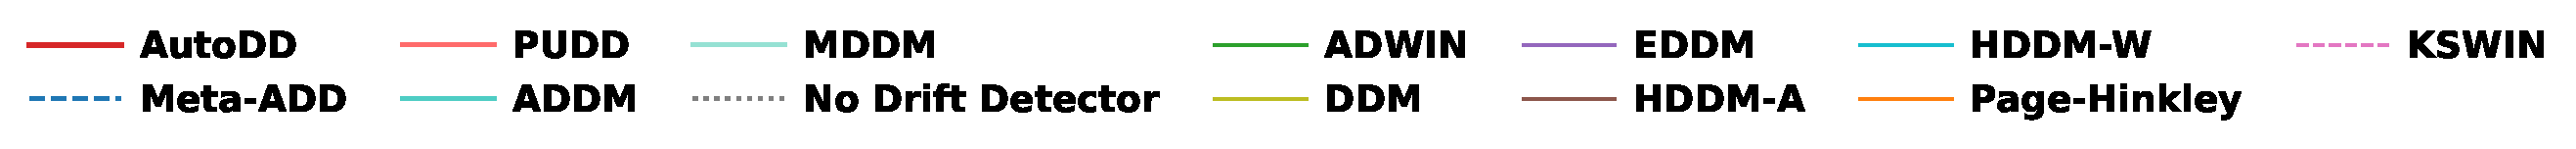
\includegraphics[width=0.95\textwidth]{images/prequential/prequential_legend.pdf}\\[4pt]
    \subfloat[SEA (GNB)\label{fig:preq_sea_gnb}]{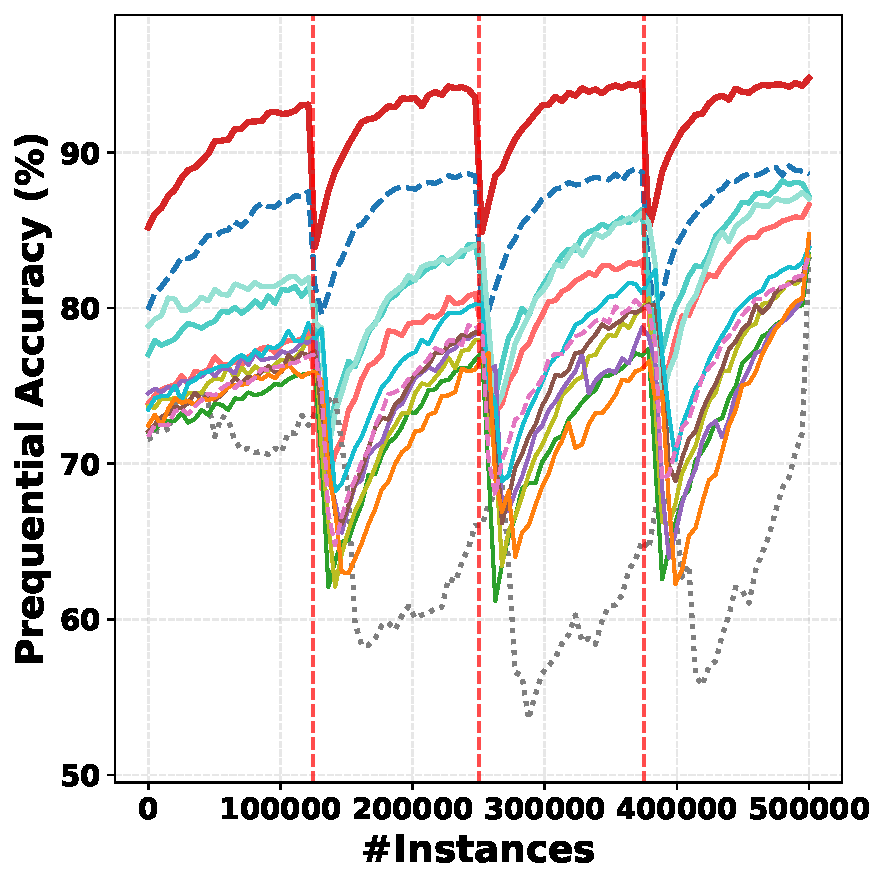
\includegraphics[width=0.24\textwidth]{images/prequential/prequential_sea_gaussiannb.pdf}}
    \hfill
    \subfloat[SEA (HAT)\label{fig:preq_sea_hat}]{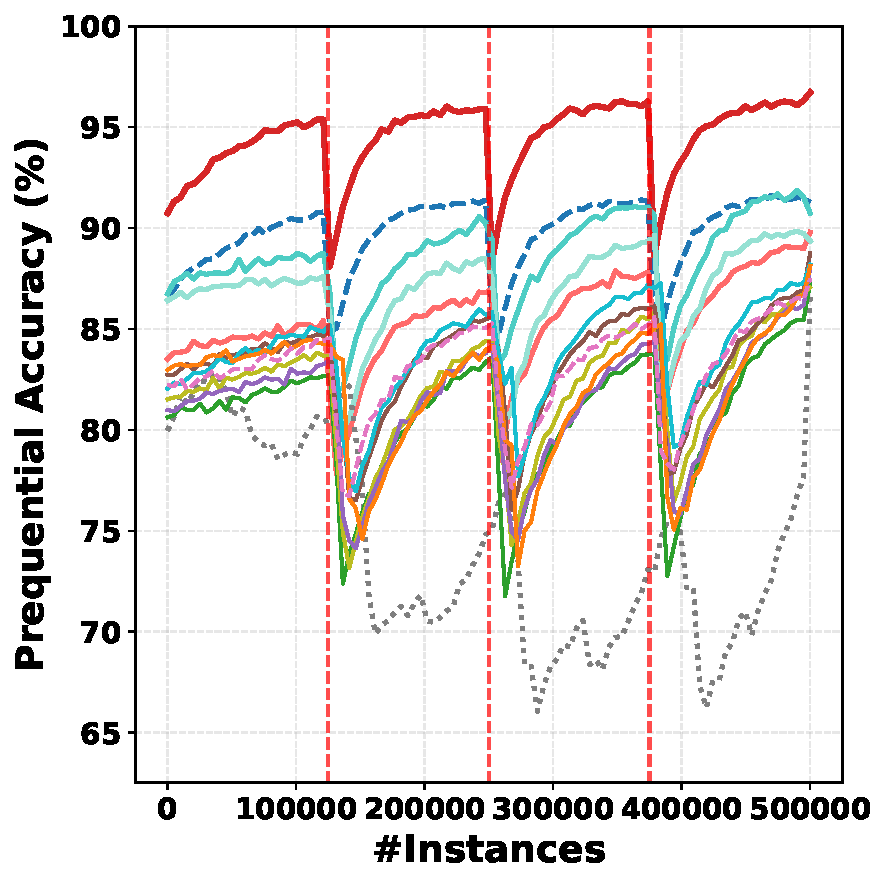
\includegraphics[width=0.24\textwidth]{images/prequential/prequential_sea_hat.pdf}}
    \hfill
    \subfloat[Poker (GNB)\label{fig:preq_poker_gnb}]{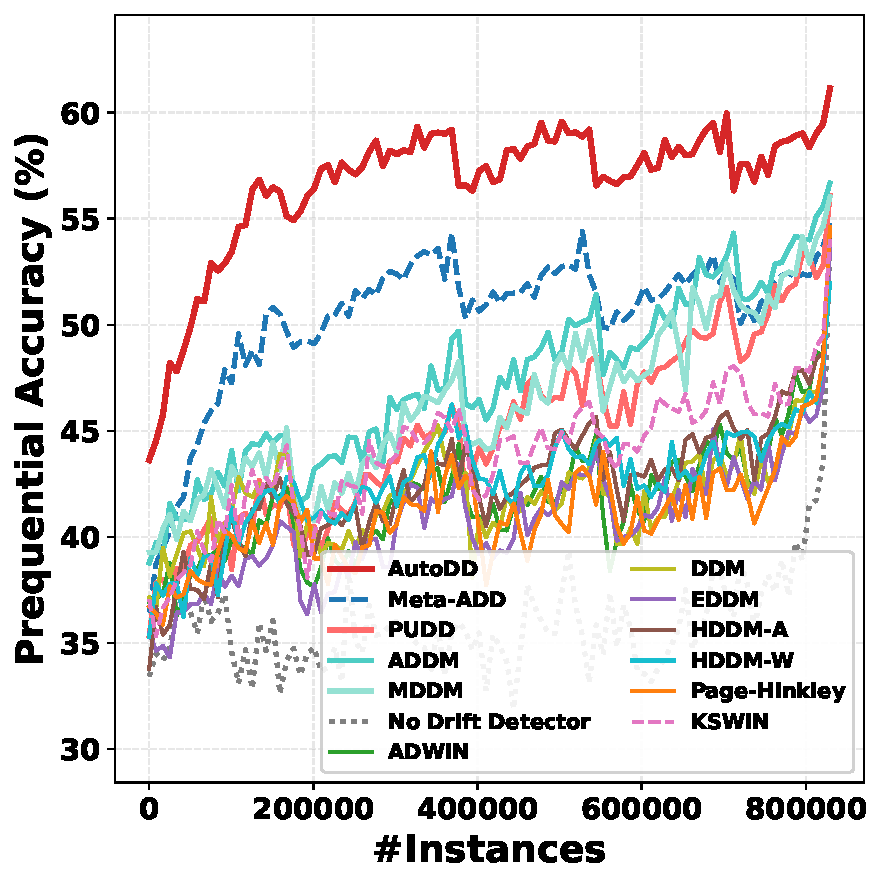
\includegraphics[width=0.24\textwidth]{images/prequential/prequential_poker_gaussiannb.pdf}}
    \hfill
    \subfloat[Poker (HAT)\label{fig:preq_poker_hat}]{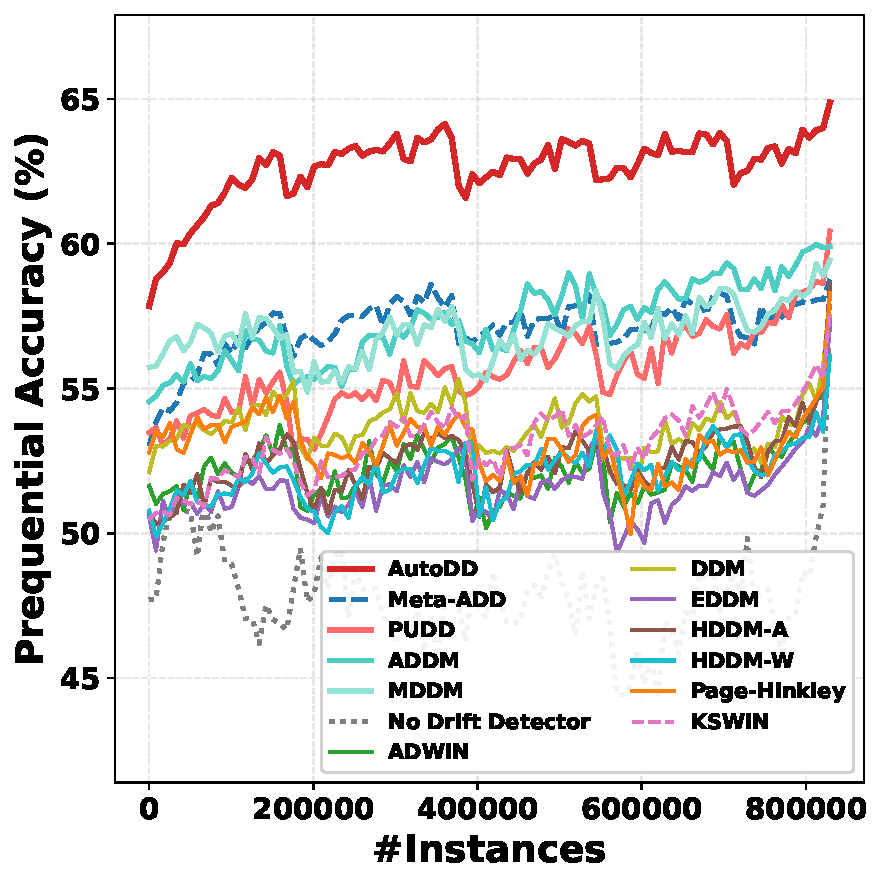
\includegraphics[width=0.24\textwidth]{images/prequential/prequential_poker_hat.pdf}}
    \caption{Prequential accuracy over time. SEA (synthetic) and Poker (real-world) datasets with GaussianNB and HAT base models.}
    \label{fig:prequential}
\end{figure*}

\subsection{Synthetic Datasets}
Tables~\ref{tab:synthetic_gnb} and~\ref{tab:synthetic_hat} compare all methods on the five synthetic benchmarks. AutoDD achieves the best mean accuracy and the best macro-F1 on every synthetic stream under both base models, with Meta-ADD ranking second across most datasets. The advantage is not uniform on accuracy. Under GaussianNB, Meta-ADD is more accurate on RBF and RTG, the two highest-dimensional streams, though AutoDD retains the better macro-F1 on both. Under HAT the macro-F1 lead over Meta-ADD is widest on these same two streams. The advantage is largest on datasets with abrupt drift, where adaptive detector switching is most beneficial, and narrows on gradual drift where Meta-ADD's learned representations are competitive. Fixed detectors exhibit inconsistent rankings across drift types, motivating the adaptive selection approach (Figures~\ref{fig:preq_sea_gnb}--\ref{fig:preq_sea_hat}).

\subsection{Real-world Datasets}
Tables~\ref{tab:realworld_gnb} and~\ref{tab:realworld_hat} report results on real-world benchmarks where drift patterns are unknown. AutoDD ranks first on mean accuracy under both base models, with the improvement consistent across all five datasets. Detection counts remain within the consensus range of the compared methods, avoiding both extremes of over- and under-detection. On Elec, Weather, and Spam, AutoDD reports the same detection count as the strongest comparators, so its accuracy gain comes from when it adapts rather than from detecting more often. Figures~\ref{fig:preq_poker_gnb} and~\ref{fig:preq_poker_hat} confirm that AutoDD tracks or leads the baselines on the Poker stream and recovers promptly after accuracy drops.

\subsection{Statistical Significance}
Figures~\ref{fig:cd_gnb} and~\ref{fig:cd_hat_main} show Critical Difference diagrams from the Friedman--Nemenyi test ($\alpha=0.05$). AutoDD achieves the best mean rank under both base models, and the No Detector baseline ranks last, confirming that drift detection is beneficial across these benchmarks. AutoDD is separated from every fixed portfolio detector by more than the critical difference, while Meta-ADD, PUDD, ADDM, and MDDM fall within the same clique.

\begin{figure}[!ht]
    \centering
    \subfloat[GaussianNB\label{fig:cd_gnb}]{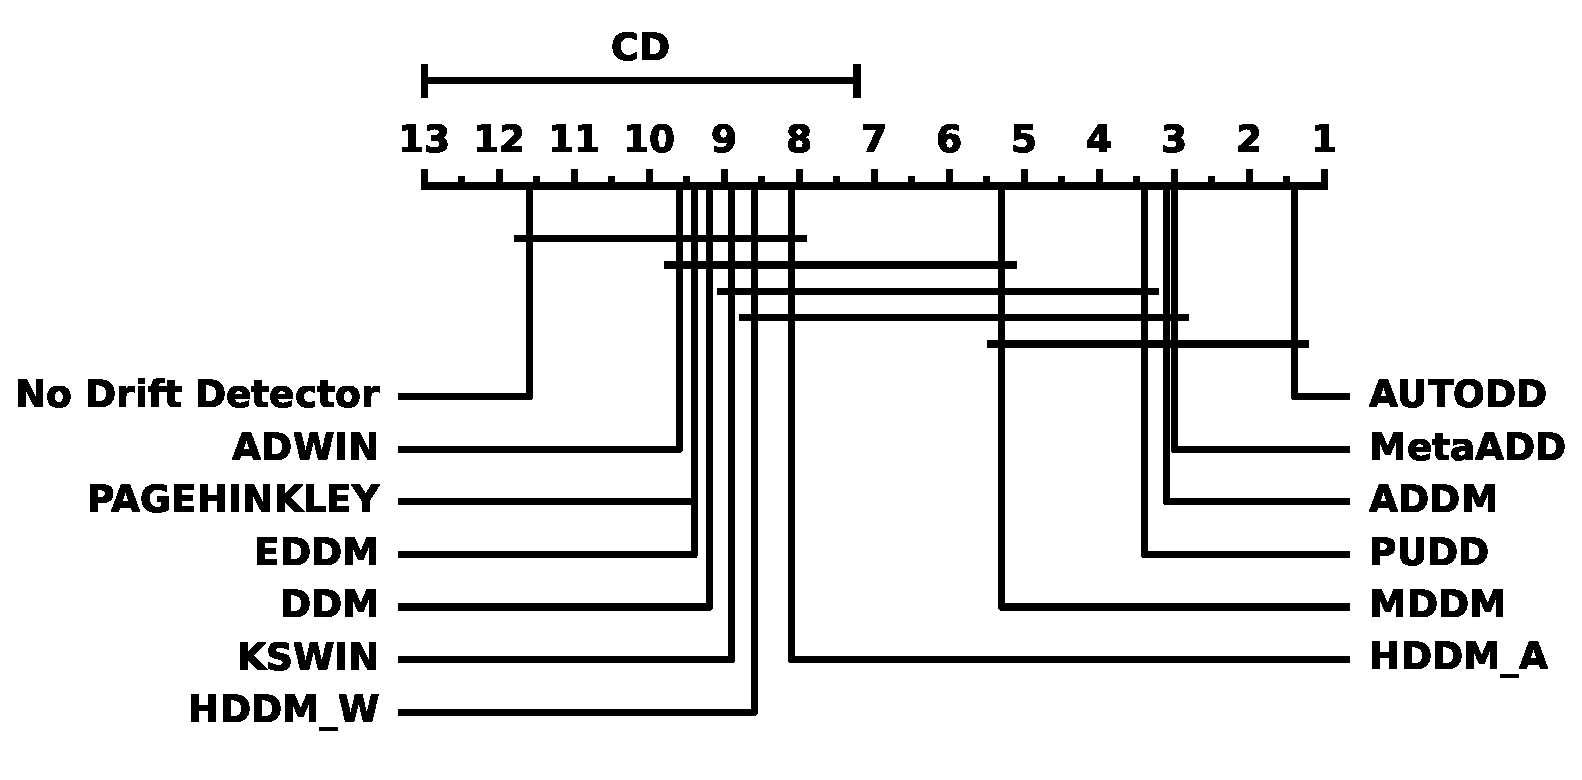
\includegraphics[width=0.48\columnwidth]{images/cd/cd_diagram_gaussiannb.pdf}}
    \hfill
    \subfloat[HAT\label{fig:cd_hat_main}]{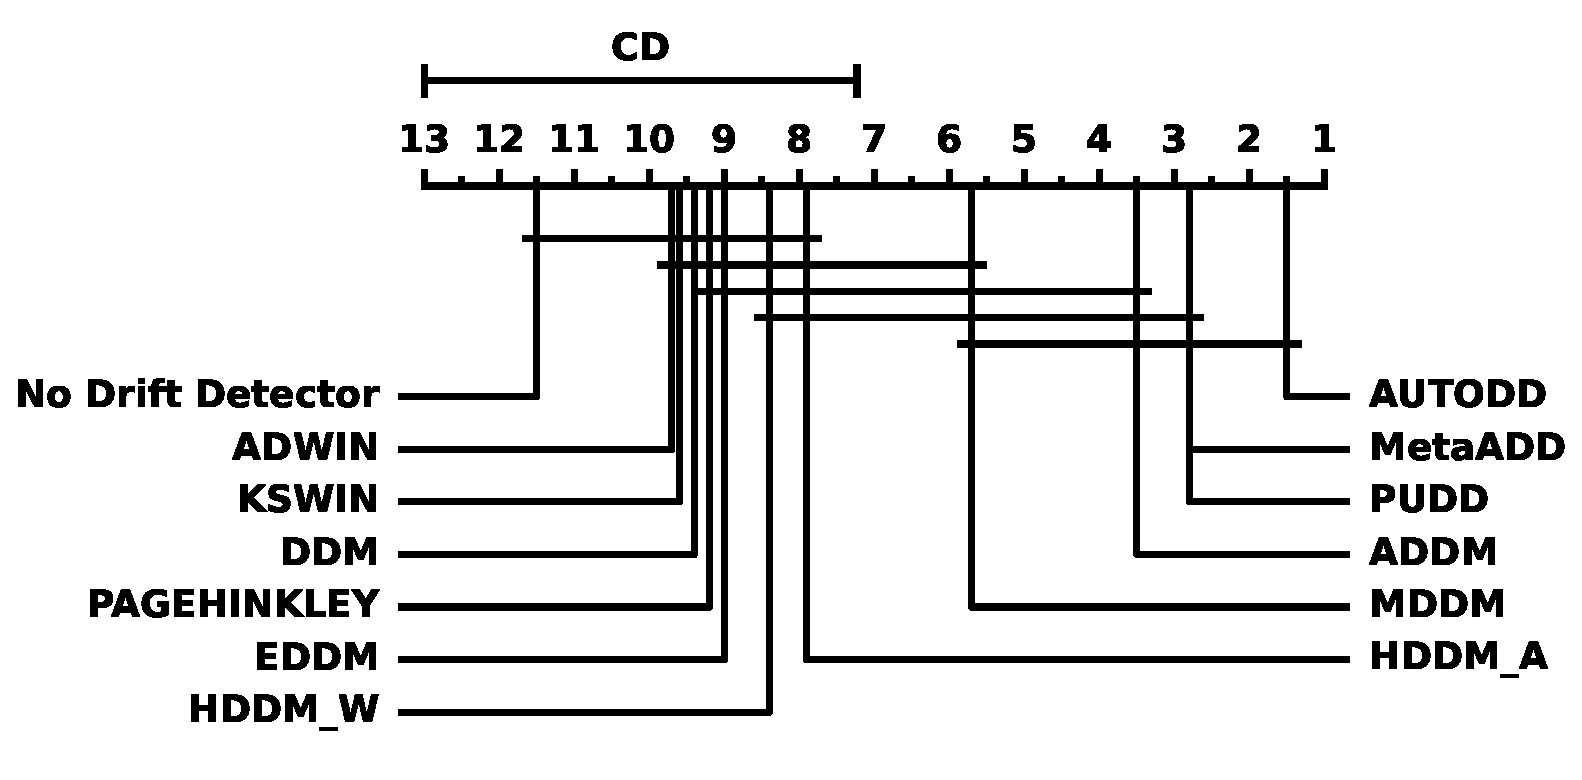
\includegraphics[width=0.48\columnwidth]{images/cd/cd_diagram_hat.pdf}}
    \caption{Critical Difference diagrams (Friedman-Nemenyi, $\alpha=0.05$). AutoDD achieves the best average rank under both base models.}
    \label{fig:cd_diagram}
\end{figure}

\subsection{Ablation Study}
Table~\ref{tab:ablation} reports performance when each component is removed in turn, using GaussianNB averaged across all datasets. Removing the Level~1 LinUCB detector selector causes the largest accuracy drop, confirming that detector-stream matching is the primary driver of adaptive performance. Removing Level~2 Thompson Sampling produces a smaller but meaningful degradation, and all three meta-feature categories provide complementary gains, with statistical features contributing most. Figure~\ref{fig:detector_selection} illustrates the resulting behaviour on the Hyperplane stream. The LinUCB layer continuously re-selects detectors as meta-features evolve, keeping the windowed error bounded and enabling rapid recovery after detected drifts.

\begin{table}[!ht]
\centering
\caption{Ablation study results (accuracy averaged across all ten datasets, macro-F1 over the five synthetic streams).}
\label{tab:ablation}
\small
\begin{tabular}{|l|c|c|c|}
\hline
\textbf{Configuration} & \textbf{Accuracy} & \textbf{Macro-F1} & \textbf{$\Delta$Acc} \\
\hline
Full AutoDD & \textbf{80.5\%} & \textbf{0.64} & -- \\
w/o Temporal & 74.2\% & 0.59 & -6.3\% \\
w/o Statistical & 71.2\% & 0.57 & -9.3\% \\
w/o Stationarity & 73.5\% & 0.59 & -7.0\% \\
w/o LinUCB (Level 1) & 62.5\% & 0.50 & -18.0\% \\
w/o Thompson (Level 2) & 75.3\% & 0.60 & -5.2\% \\
\hline
\end{tabular}
\end{table}

\begin{figure}[!ht]
    \centering
    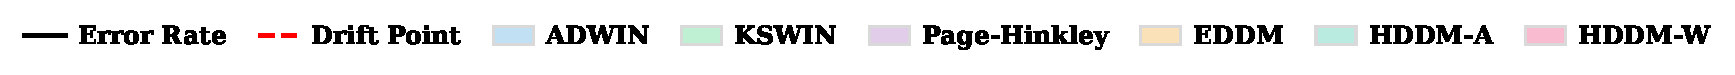
\includegraphics[width=\columnwidth]{images/selection/detector_selection_legend_hyp.pdf}\\[2pt]
    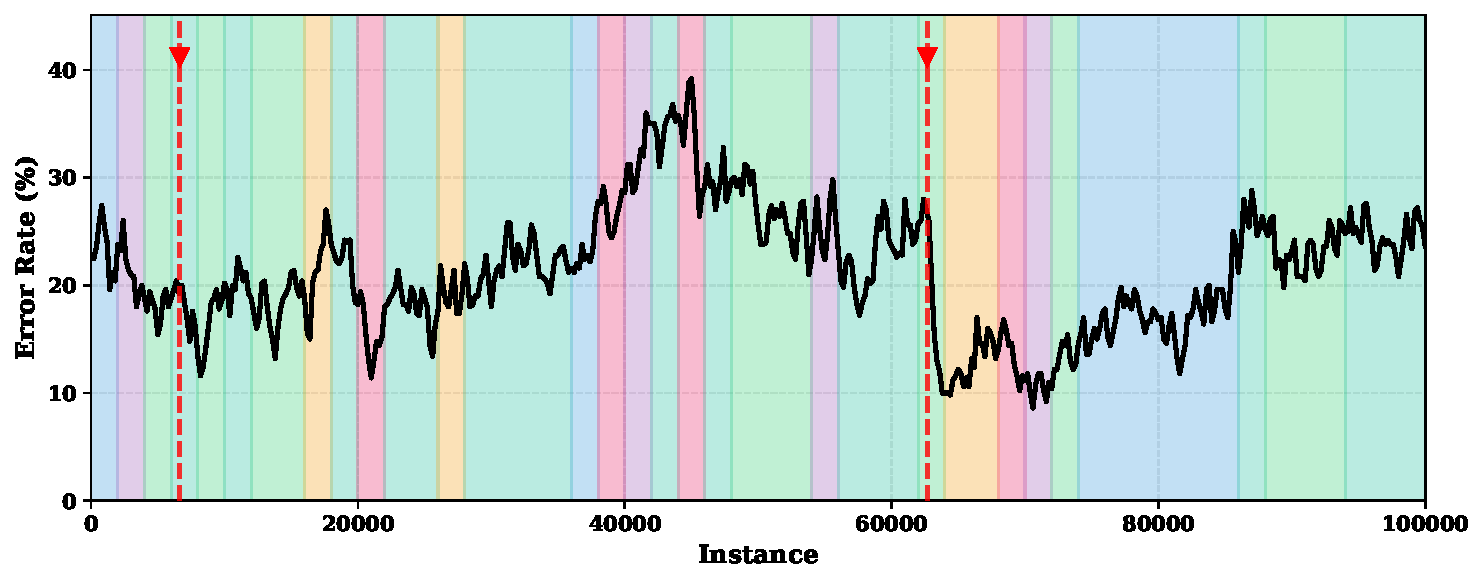
\includegraphics[width=\columnwidth]{images/selection/detector_selection_hyp.pdf}
    \caption{Detector selection by AutoDD over the first 100{,}000 instances of the Hyperplane stream. All quantitative results use the full 500{,}000-instance stream. Coloured bands show the dominant LinUCB-selected detector per block, the black curve the windowed prequential error rate, and dashed red lines the drift alarms raised by AutoDD, not ground-truth drift points.}
    \label{fig:detector_selection}
\end{figure}

\subsection{Sensitivity Study}
Figure~\ref{fig:sensitivity} shows AutoDD's sensitivity to its three key hyperparameters. Performance peaks at $w=100$, where smaller windows introduce high variance and larger windows delay drift response. The exploration parameter $\alpha_{\text{ucb}}$ shows a clear optimum, with under-exploration causing exploitation bias and over-exploration reducing accuracy. The regularisation parameter $\lambda_{\text{reg}}$ is robust across the tested range, and AutoDD degrades gracefully around the default settings.

\begin{figure}[!ht]
    \centering
    \subfloat[$w$\label{fig:window_sensitivity}]{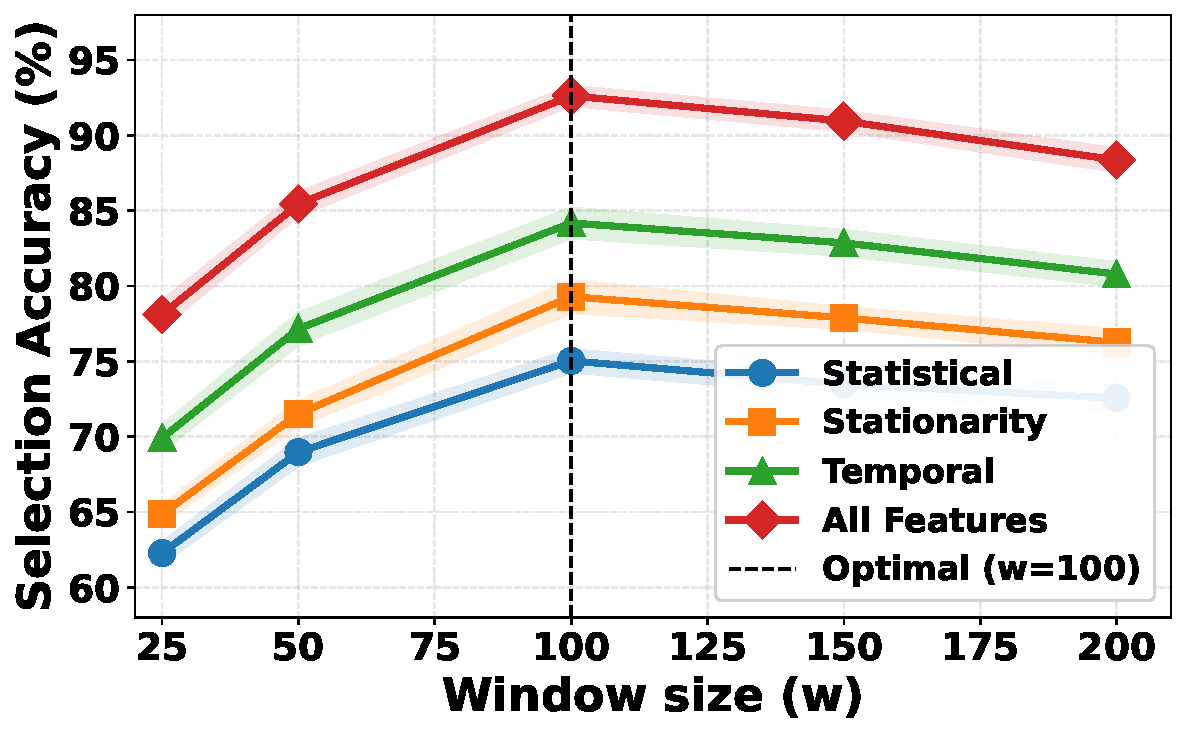
\includegraphics[width=0.32\columnwidth]{images/sensitivity/window_sensitivity.pdf}}
    \hfill
    \subfloat[$\alpha_{\text{ucb}}$\label{fig:alpha_sensitivity}]{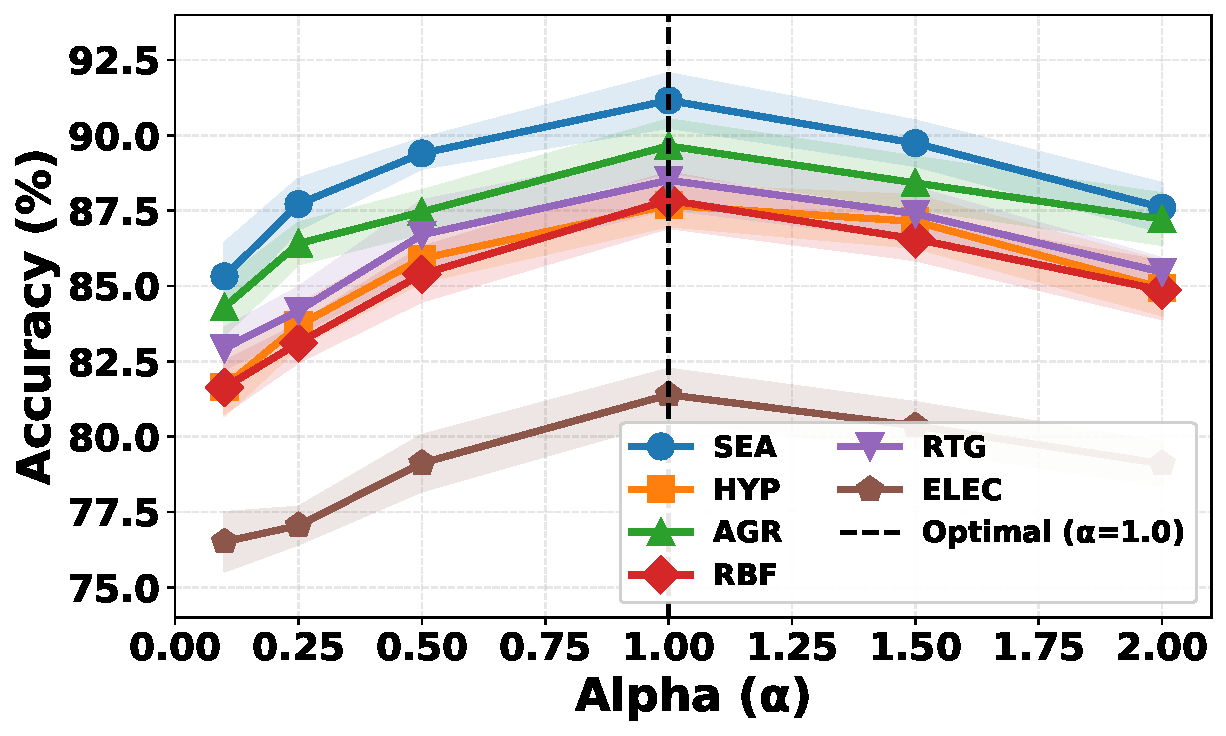
\includegraphics[width=0.32\columnwidth]{images/sensitivity/alpha_sensitivity.pdf}}
    \hfill
    \subfloat[$\lambda_{\text{reg}}$\label{fig:lambda_sensitivity}]{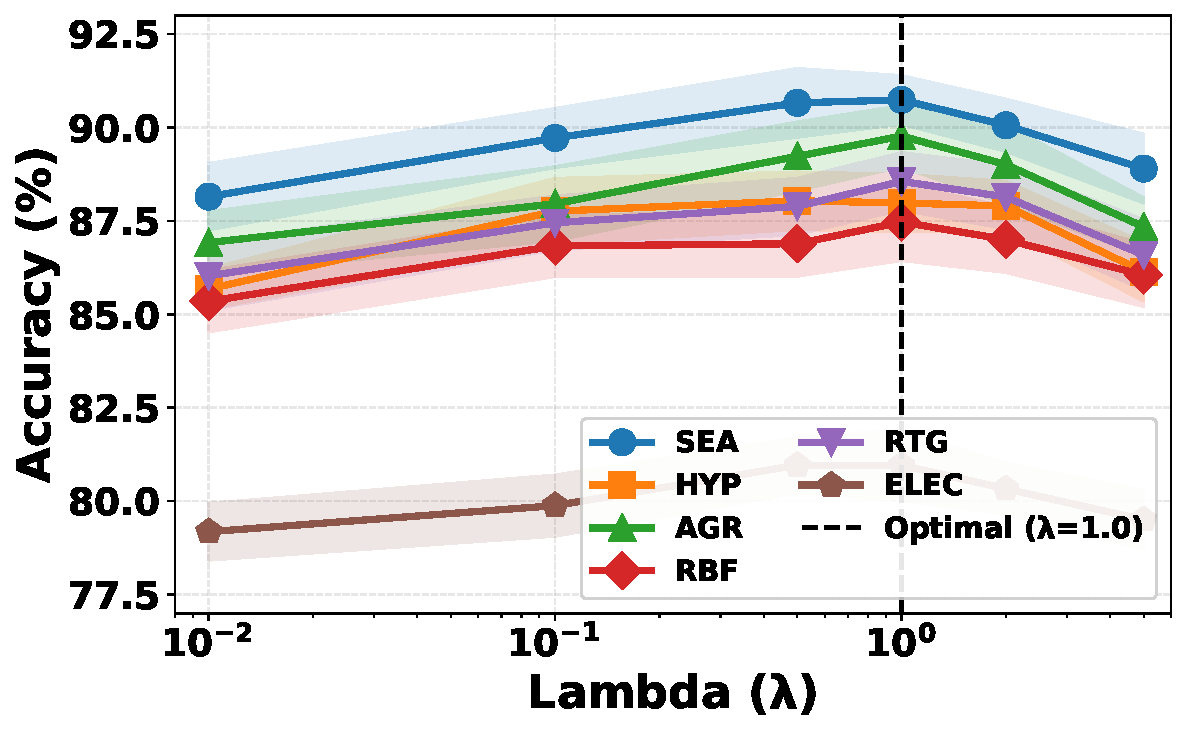
\includegraphics[width=0.32\columnwidth]{images/sensitivity/lambda_sensitivity.pdf}}
    \caption{Hyperparameter sensitivity analysis showing selection accuracy across different values of (a) window size $w$, (b) exploration parameter $\alpha_{\text{ucb}}$, and (c) regularisation parameter $\lambda_{\text{reg}}$.}
    \label{fig:sensitivity}
\end{figure}

\subsection{Computational Efficiency}
Figures~\ref{fig:tm_gnb} and~\ref{fig:tm_hat} place all methods in the runtime-memory plane. AutoDD occupies the fast, low-memory region under both base models, with the hierarchical selection mechanism introducing only modest overhead. It is strictly more efficient than Meta-ADD and PUDD while delivering better detection performance, making it practical for high-velocity streams.

\begin{figure}[!ht]
    \centering
    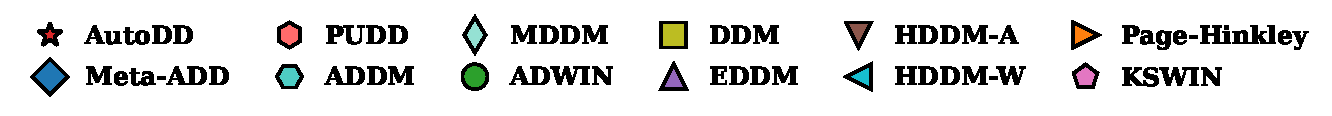
\includegraphics[width=\columnwidth]{images/efficiency/time_memory_legend.pdf}\\[3pt]
    \subfloat[GaussianNB\label{fig:tm_gnb}]{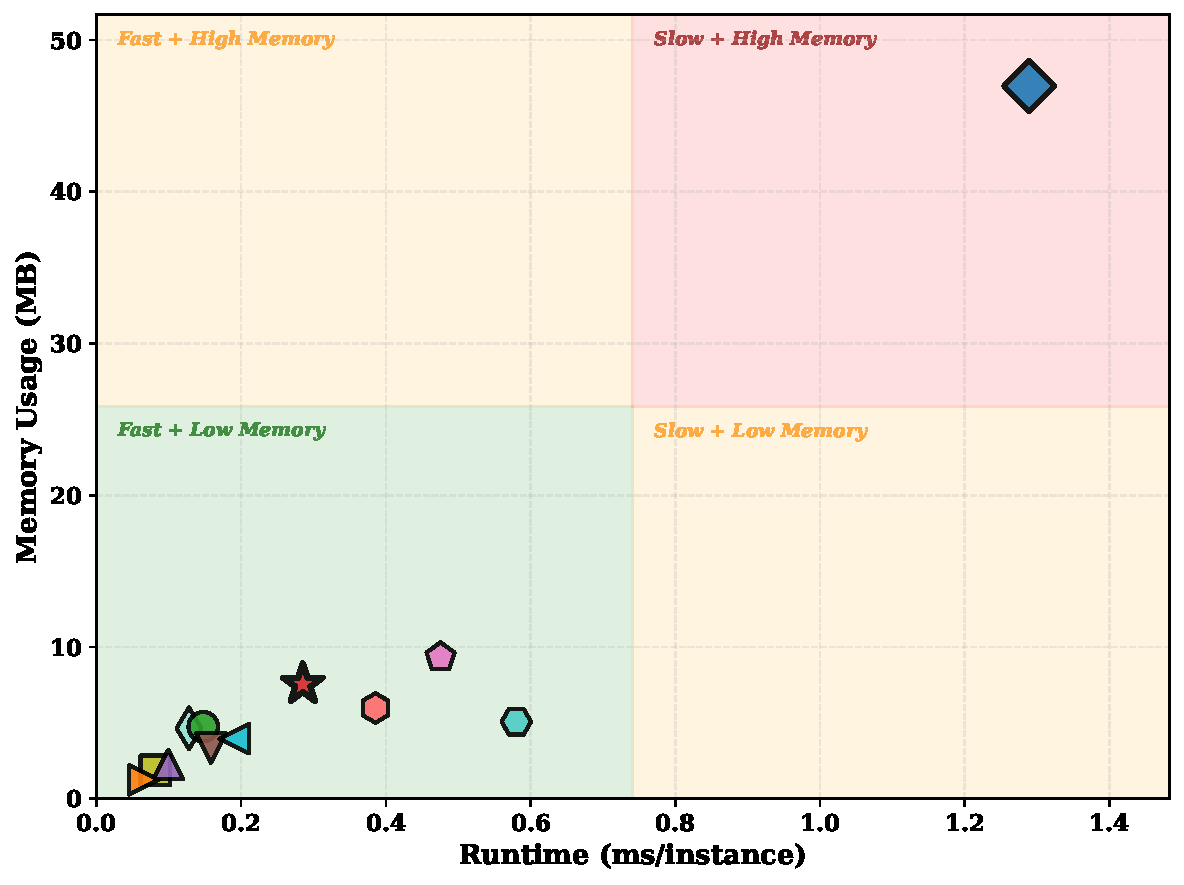
\includegraphics[width=0.48\columnwidth]{images/efficiency/time_memory_gaussiannb.pdf}}
    \hfill
    \subfloat[HAT\label{fig:tm_hat}]{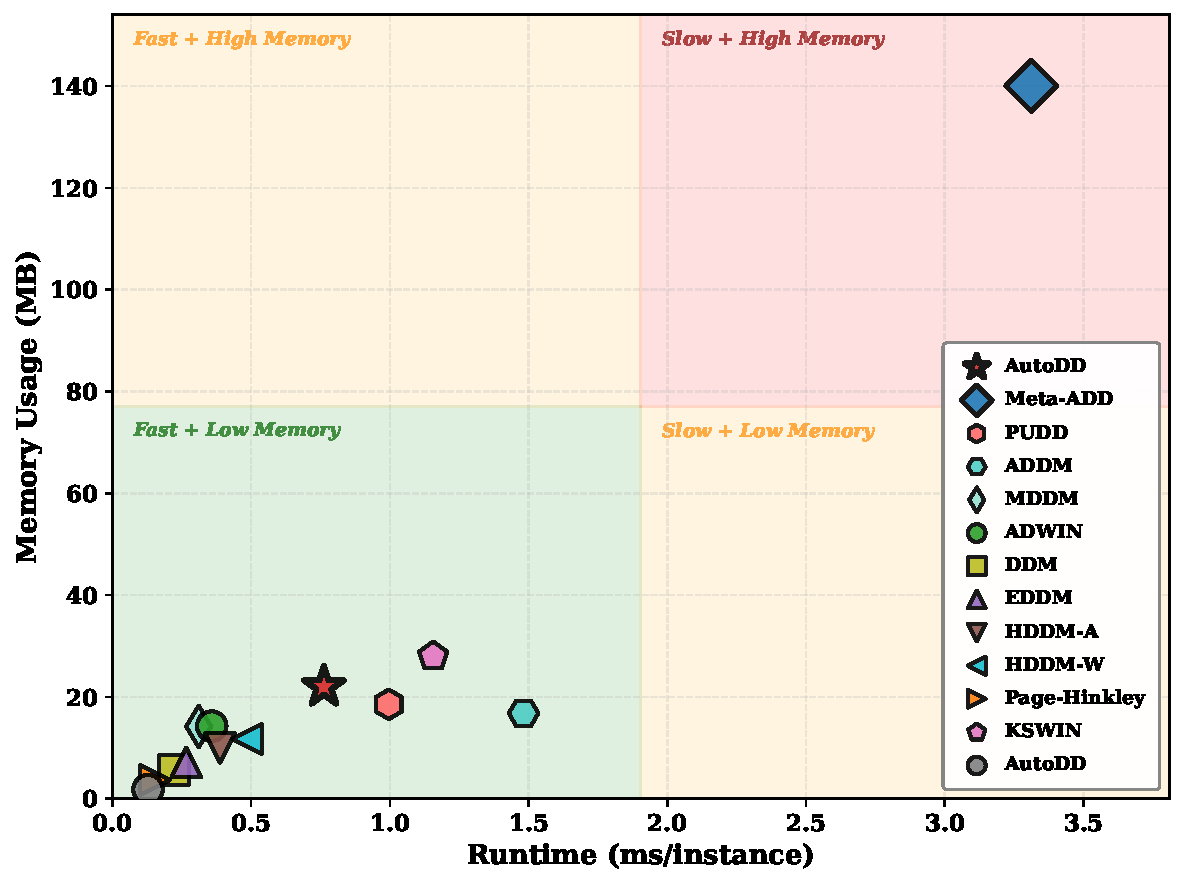
\includegraphics[width=0.48\columnwidth]{images/efficiency/time_memory_hat.pdf}}
    \caption{Runtime vs. memory trade-off. AutoDD lies in the Fast + Low Memory quadrant under both base models.}
    \label{fig:time_memory}
\end{figure}


\section{Discussion and Limitations}
\label{sec:discussion}
We highlight several boundaries of the current design. First, AutoDD automates detector and hyperparameter selection but not the sliding-window size, which the sensitivity analysis shows to be the most influential setting. The default value is robust across our benchmarks, yet selecting it for an unseen stream remains a manual step that an outer adaptive loop could close. Second, the reward is an accuracy-based proxy and therefore entangles detector quality with the downstream learner. We mitigate this through window-level smoothing and the significance threshold, and empirical results confirm that selection preferences are consistent across base learners, though a fully label-free reward remains an open direction. Third, to isolate detection from model selection we fix the base learner to GaussianNB and HAT, which are two standard but limited families, and adapt via full model reset, while richer learners and softer adaptation strategies (warm-starting, selective parameter resets, replay, ensemble updating) are left to future work. Fourth, the comparison is asymmetric in two respects that temper the reported margins. The four strongest comparators (MDDM, ADDM, PUDD, and Meta-ADD) are evaluated as baselines but are not members of the portfolio AutoDD selects from, so the action space is restricted to the classical detectors of Table~\ref{tab:portfolio}. In addition, all baselines run at fixed literature-recommended hyperparameters while AutoDD tunes its detector online, so part of its advantage is attributable to tuning rather than to selection. Separating these two effects requires a comparator granted an equivalent tuning budget, which we leave to future work. Finally, AutoDD targets tabular data streams, the prevalent setting in the drift-detection literature. Non-tabular modalities such as image, audio, and text are outside the scope of this work \cite{Souza2021IBDD}.

\section{Conclusion and Future Work}
\label{sec:conclusion}

This paper addressed a component that streaming AutoML has so far left to manual specification, namely the drift detector itself. We formalised the joint choice of detector and hyperparameters as a contextual selection problem and introduced AutoDD, which solves it online with a two-level hierarchical bandit. Level~1 uses LinUCB over 15 online meta-features to select a detector, and Level~2 uses Thompson Sampling to select its configuration, both driven by a bounded proxy reward because no drift labels are available at run time. Across ten benchmarks and two base learners, AutoDD attains the best mean accuracy and macro-F1 and the best average rank under the Friedman--Nemenyi test, while the ablation confirms detector selection as the main driver and its runtime and memory stay in the fast, low-memory region.

Several directions follow from the limitations of Section~\ref{sec:discussion}. The most immediate is learning the window size $w$ in an outer adaptive loop, since the sensitivity analysis identifies it as the most influential setting. A second is replacing the accuracy-based proxy with a label-free reward that decouples detector credit from the downstream learner. A third is broadening the portfolio and granting baselines an equivalent tuning budget, separating the benefit of selection from that of tuning. Finally, evaluating on streams with annotated change points would allow detection delay and false alarms to be scored directly.

\bibliographystyle{IEEEtran}
\bibliography{references}

% ============================================================
\appendix
% ============================================================

\section{Additional Results}\label{appendix:additional_results}

\begin{figure}[!ht]
\centering
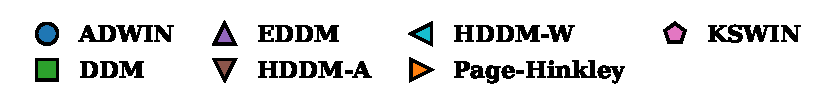
\includegraphics[width=0.65\columnwidth]{images/reward/reward_consistency_legend.pdf}\\
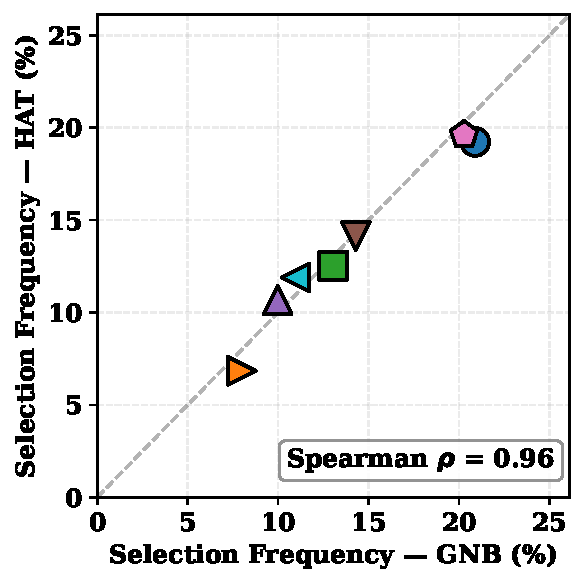
\includegraphics[width=0.65\columnwidth]{images/reward/reward_consistency.pdf}
\caption{Mean detector selection frequency under GaussianNB against HAT across all ten datasets. Every detector lies near the diagonal (Spearman $\rho=0.96$, $p<0.001$), indicating that the proxy reward tracks detector quality rather than base-learner artefacts.}
\label{fig:reward_consistency}
\end{figure}

\begin{table}[!ht]
\centering
\caption{Accuracy (\%) broken down by drift type under GaussianNB. AutoDD leads on sudden, incremental, and recurring drift, while Meta-ADD edges ahead on gradual drift owing to its learned drift-type representations.}
\label{tab:drift_type}
\resizebox{\columnwidth}{!}{%
\small
\begin{tabular}{|l|c|c|c|c|}
\hline
\textbf{Method} & \textbf{Sudden} & \textbf{Gradual} & \textbf{Incremental} & \textbf{Recurring} \\
\hline
ADWIN & 82.4 & 71.3 & 68.5 & 75.2 \\
DDM & 79.8 & 74.6 & 72.1 & 71.8 \\
EDDM & 75.2 & 78.4 & 74.8 & 69.3 \\
HDDM-A & 81.7 & 72.1 & 69.8 & 74.5 \\
HDDM-W & 80.1 & 76.2 & 73.5 & 74.6 \\
Page-Hinkley & 81.9 & 70.8 & 68.2 & 75.8 \\
KSWIN & 76.5 & 77.8 & 75.2 & 72.1 \\
MDDM & 81.3 & 75.8 & 74.1 & 73.9 \\
ADDM & 82.9 & 77.2 & 75.6 & 74.8 \\
PUDD & 82.1 & 79.5 & 76.8 & 75.4 \\
Meta-ADD & 84.6 & \textbf{82.3} & 78.9 & 77.8 \\
\textbf{AutoDD} & \textbf{88.2} & 81.7 & \textbf{80.4} & \textbf{79.6} \\
\hline
\end{tabular}
}
\end{table}


\begin{table}[!ht]
\centering
\caption{Detector selection frequency (\%) by stream characteristic. The learned policy aligns with domain knowledge, favouring ADWIN and DDM on high-velocity streams and KSWIN on high-noise and high-dimensional streams.}
\label{tab:selection_pattern}
\small
\begin{tabular}{|l|c|c|c|}
\hline
\textbf{Detector} & \textbf{High Velocity} & \textbf{High Noise} & \textbf{High Dim.} \\
\hline
ADWIN & 28.4 & 12.3 & 15.7 \\
DDM & 22.1 & 8.5 & 11.2 \\
EDDM & 8.3 & 18.7 & 14.5 \\
HDDM-A & 15.2 & 10.4 & 12.8 \\
HDDM-W & 12.6 & 14.2 & 13.1 \\
Page-Hinkley & 5.8 & 8.1 & 7.2 \\
KSWIN & 7.6 & 27.8 & 25.5 \\
\hline
\end{tabular}
\end{table}


\begin{table}[!ht]
\centering
\caption{Mean detection delay (instances) on the synthetic datasets, lower is better. AutoDD attains the lowest delay of all comparators, selecting responsive detectors during drift-prone windows while avoiding over-sensitive choices in stable periods.}
\label{tab:delay_main}
\small
\begin{tabular}{|l|c|c|c|c|c|}
\hline
\textbf{Method} & \textbf{SEA} & \textbf{HYP} & \textbf{AGR} & \textbf{RBF} & \textbf{Mean} \\
\hline
ADWIN & 45.2 & 78.3 & 52.1 & 81.4 & 64.3 \\
DDM & 38.7 & 62.5 & 48.9 & 65.2 & 53.8 \\
EDDM & 52.3 & 71.8 & 61.4 & 74.6 & 65.0 \\
HDDM-A & 43.8 & 75.1 & 50.3 & 78.6 & 61.9 \\
HDDM-W & 41.5 & 58.2 & 45.7 & 62.8 & 52.1 \\
Page-Hinkley & 46.9 & 80.5 & 53.8 & 83.2 & 66.1 \\
KSWIN & 49.1 & 68.7 & 58.2 & 71.4 & 61.9 \\
MDDM & 39.4 & 55.8 & 44.2 & 60.5 & 50.0 \\
ADDM & 36.5 & 51.3 & 41.6 & 57.8 & 46.8 \\
PUDD & 32.8 & 45.2 & 37.5 & 51.6 & 41.8 \\
Meta-ADD & 35.2 & 48.6 & 39.8 & 55.3 & 44.7 \\
\textbf{AutoDD} & \textbf{28.4} & \textbf{42.1} & \textbf{34.2} & \textbf{48.7} & \textbf{38.4} \\
\hline
\end{tabular}
\end{table}


\begin{table}[!ht]
\centering
\caption{AutoDD proxy-oracle selection agreement (\%) by stream quarter. Agreement rises monotonically from the first to the final quarter on every dataset, showing that the LinUCB layer learns reliable detector selections from the reward signal as the stream progresses.}
\label{tab:conv_main}
\small
\begin{tabular}{|l|c|c|c|c|}
\hline
\textbf{Dataset} & \textbf{0--25\%} & \textbf{25--50\%} & \textbf{50--75\%} & \textbf{75--100\%} \\
\hline
SEA   & 71.2 & 85.4 & 91.8 & 94.3 \\
HYP   & 68.5 & 82.1 & 89.6 & 93.1 \\
AGR   & 65.8 & 79.3 & 87.2 & 91.5 \\
Elec  & 72.4 & 84.7 & 90.3 & 92.8 \\
Poker & 69.1 & 81.6 & 88.9 & 93.6 \\
\textbf{Mean} & 69.4 & 82.6 & 89.6 & 93.1 \\
\hline
\end{tabular}
\end{table}



% \section{Meta-Feature Formulations}\label{appendix:metafeatures}

\begin{table}[!ht]
\centering
\caption{AutoDD hyperparameter settings used in all experiments, for reproducibility. Detector-specific hyperparameter ranges and defaults are given in Table~\ref{tab:portfolio}.}
\label{tab:reproducibility}
\resizebox{\columnwidth}{!}{%
\small
\begin{tabular}{|l|l|c|}
\hline
\textbf{Component} & \textbf{Parameter} & \textbf{Value} \\
\hline
\multirow{2}{*}{Stream} & Window size $w$ & 100 \\
\cline{2-3}
& Meta-feature dimensionality $m$ & 15 \\
\hline
\multirow{2}{*}{Portfolio} & Number of detectors $K$ & 7 \\
\cline{2-3}
& Configurations per detector $C$ & 5 \\
\hline
\multirow{2}{*}{Level 1 (LinUCB)} & Exploration $\alpha_{\text{ucb}}$ & 1.0 \\
\cline{2-3}
& Regularisation $\lambda_{\text{reg}}$ & 1.0 \\
\hline
Level 2 (Thompson) & Beta prior $(a_0, b_0)$ & $(1, 1)$ \\
\hline
\multirow{6}{*}{Reward (Eq.~\eqref{eq:reward})} & Significance threshold $\tau_{\text{sig}}$ & 0.05 \\
\cline{2-3}
& True-positive base $\rho_{\mathrm{tp}}$ & 0.5 \\
\cline{2-3}
& Accuracy-drop scale $\kappa$ & 2 \\
\cline{2-3}
& False-positive penalty $\rho_{\mathrm{fp}}$ & 0.3 \\
\cline{2-3}
& False-negative base $\rho_{\mathrm{fn}}$ & 0.5 \\
\cline{2-3}
& True-negative reward $\rho_{\mathrm{tn}}$ & 0.1 \\
\hline
\multirow{2}{*}{Evaluation} & Runs per dataset & 10 \\
\cline{2-3}
& Random seeds & $\sim \mathcal{U}\{1, \ldots, 100\}$ \\
\hline
\end{tabular}
}
\end{table}

\begin{table}[!ht]
\centering
\caption{The 15 online meta-features forming the context vector $\boldsymbol{\phi}_t$, grouped by category, with the closed-form expression or online estimator used to compute each over the sliding window of size $w$.}
\label{tab:metafeatures}
\resizebox{\columnwidth}{!}{%
\small
\begin{tabular}{|l|l|l|}
\hline
\textbf{Category} & \textbf{Feature} & \textbf{Formula/Description} \\
\hline
\multirow{5}{*}{Statistical} & Velocity & $v_t = n_t/\Delta t$ \\
& Dimensionality & $d$ \\
& Sparsity & $\frac{1}{wd}\sum_{i=1}^{w}\sum_{j=1}^{d}\mathbb{I}[\mathbf{x}_{i,j}=0]$ \\
& Noise level & $H(\mathbf{X}) \approx -\frac{1}{w}\sum_{i=1}^{w}\log \hat{p}_k(\mathbf{x}_i)$ (k-NN, $k=5$) \\
& Class imbalance & $\max_c |C_c| / \min_c |C_c|$ \\
\hline
\multirow{5}{*}{Stationarity} & Error volatility & $\sigma_{\text{err}}(t) = \sqrt{\frac{1}{w}\sum_{i=t-w}^{t}(e_i - \bar{e})^2}$ \\
& KL divergence & $D_{\text{KL}}(P_t \| P_{t-1})$ (histogram, $\sqrt{w}$ bins) \\
& Autocorrelation & $\rho_t = \frac{\text{Cov}(e_t, e_{t-1})}{\sigma_{e_t}\sigma_{e_{t-1}}}$ \\
& Mean shift & $\Delta\mu_t = \frac{1}{d}\sum_{j=1}^{d}|\mu_{t,j} - \mu_{t-1,j}|$ \\
& Variance shift & $\Delta\sigma^2_t = \frac{1}{d}\sum_{j=1}^{d}|\sigma^2_{t,j} - \sigma^2_{t-1,j}|$ \\
\hline
\multirow{5}{*}{Temporal} & Trend & $\beta_{\text{trend}} = \frac{\text{Cov}(t, e_t)}{\text{Var}(t)}$ \\
& Periodicity & $f_{\text{dom}} = \arg\max_f |\mathcal{F}\{e_t\}(f)|$ \\
& Change frequency & $\frac{1}{\Delta t}\sum_{i=1}^{w}\mathbb{I}[|\Delta e_i| > \tau_{\Delta e}]$ \\
& Change magnitude & $\frac{1}{|\mathcal{C}_t|}\sum_{i \in \mathcal{C}_t}|\Delta e_i|$ \\
& Recurrence score & $\frac{1}{w^2}\sum_{i,j}\mathbb{I}[\|\mathbf{x}_i - \mathbf{x}_j\| < \epsilon]$ \\
\hline
\end{tabular}
}
\end{table}

\end{document}
